\chapter{Projekt}

\section{Przypadki użycia}
\todo{diagram przypadków użycia}

\begin{minipage}{\textwidth}
    \begin{figure}[H]
        \centering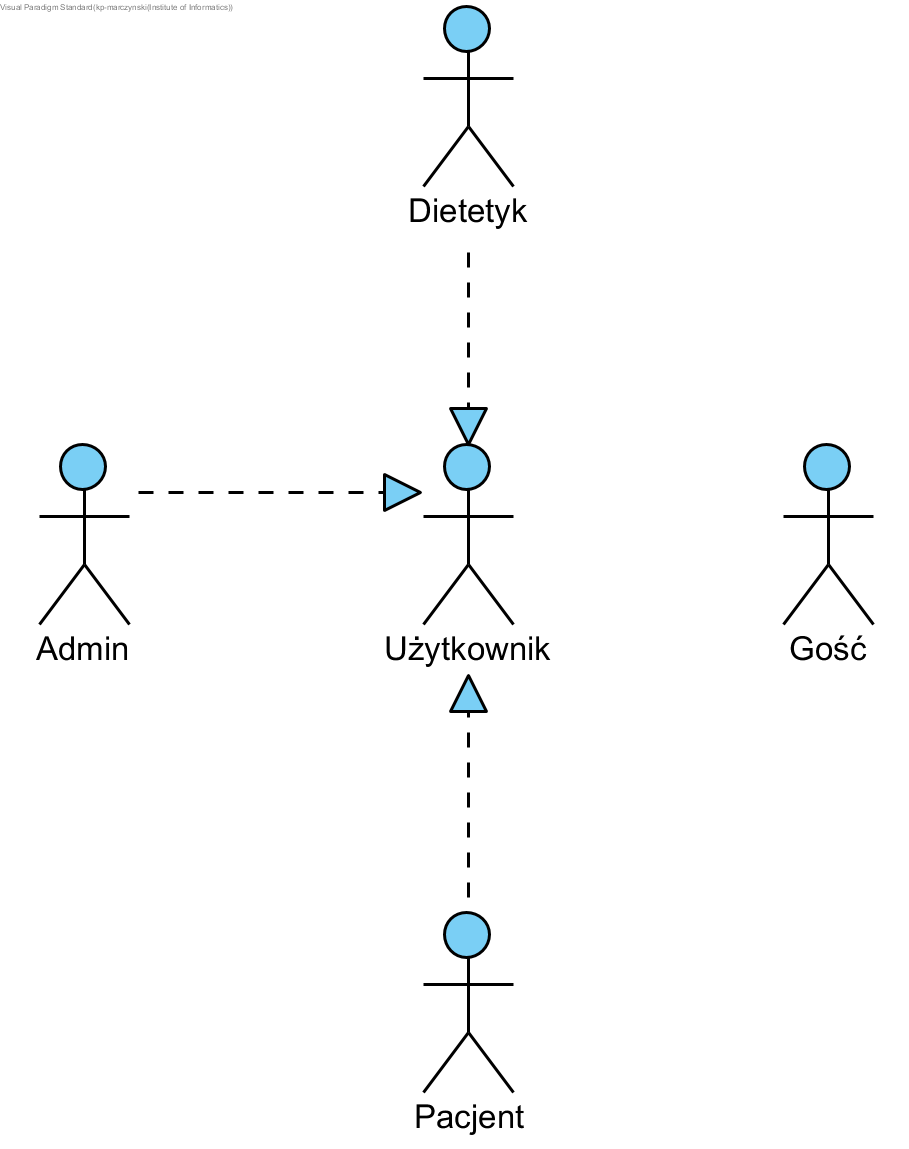
\includegraphics[scale=0.4]{../uml/use_case_diagrams/users.png}
        \caption{Typy danych (opr.wł).}\label{rysunek:use-case-diagram-data-types}
    \end{figure}
\end{minipage}

\begin{minipage}{\textwidth}
    \begin{figure}[H]
        \centering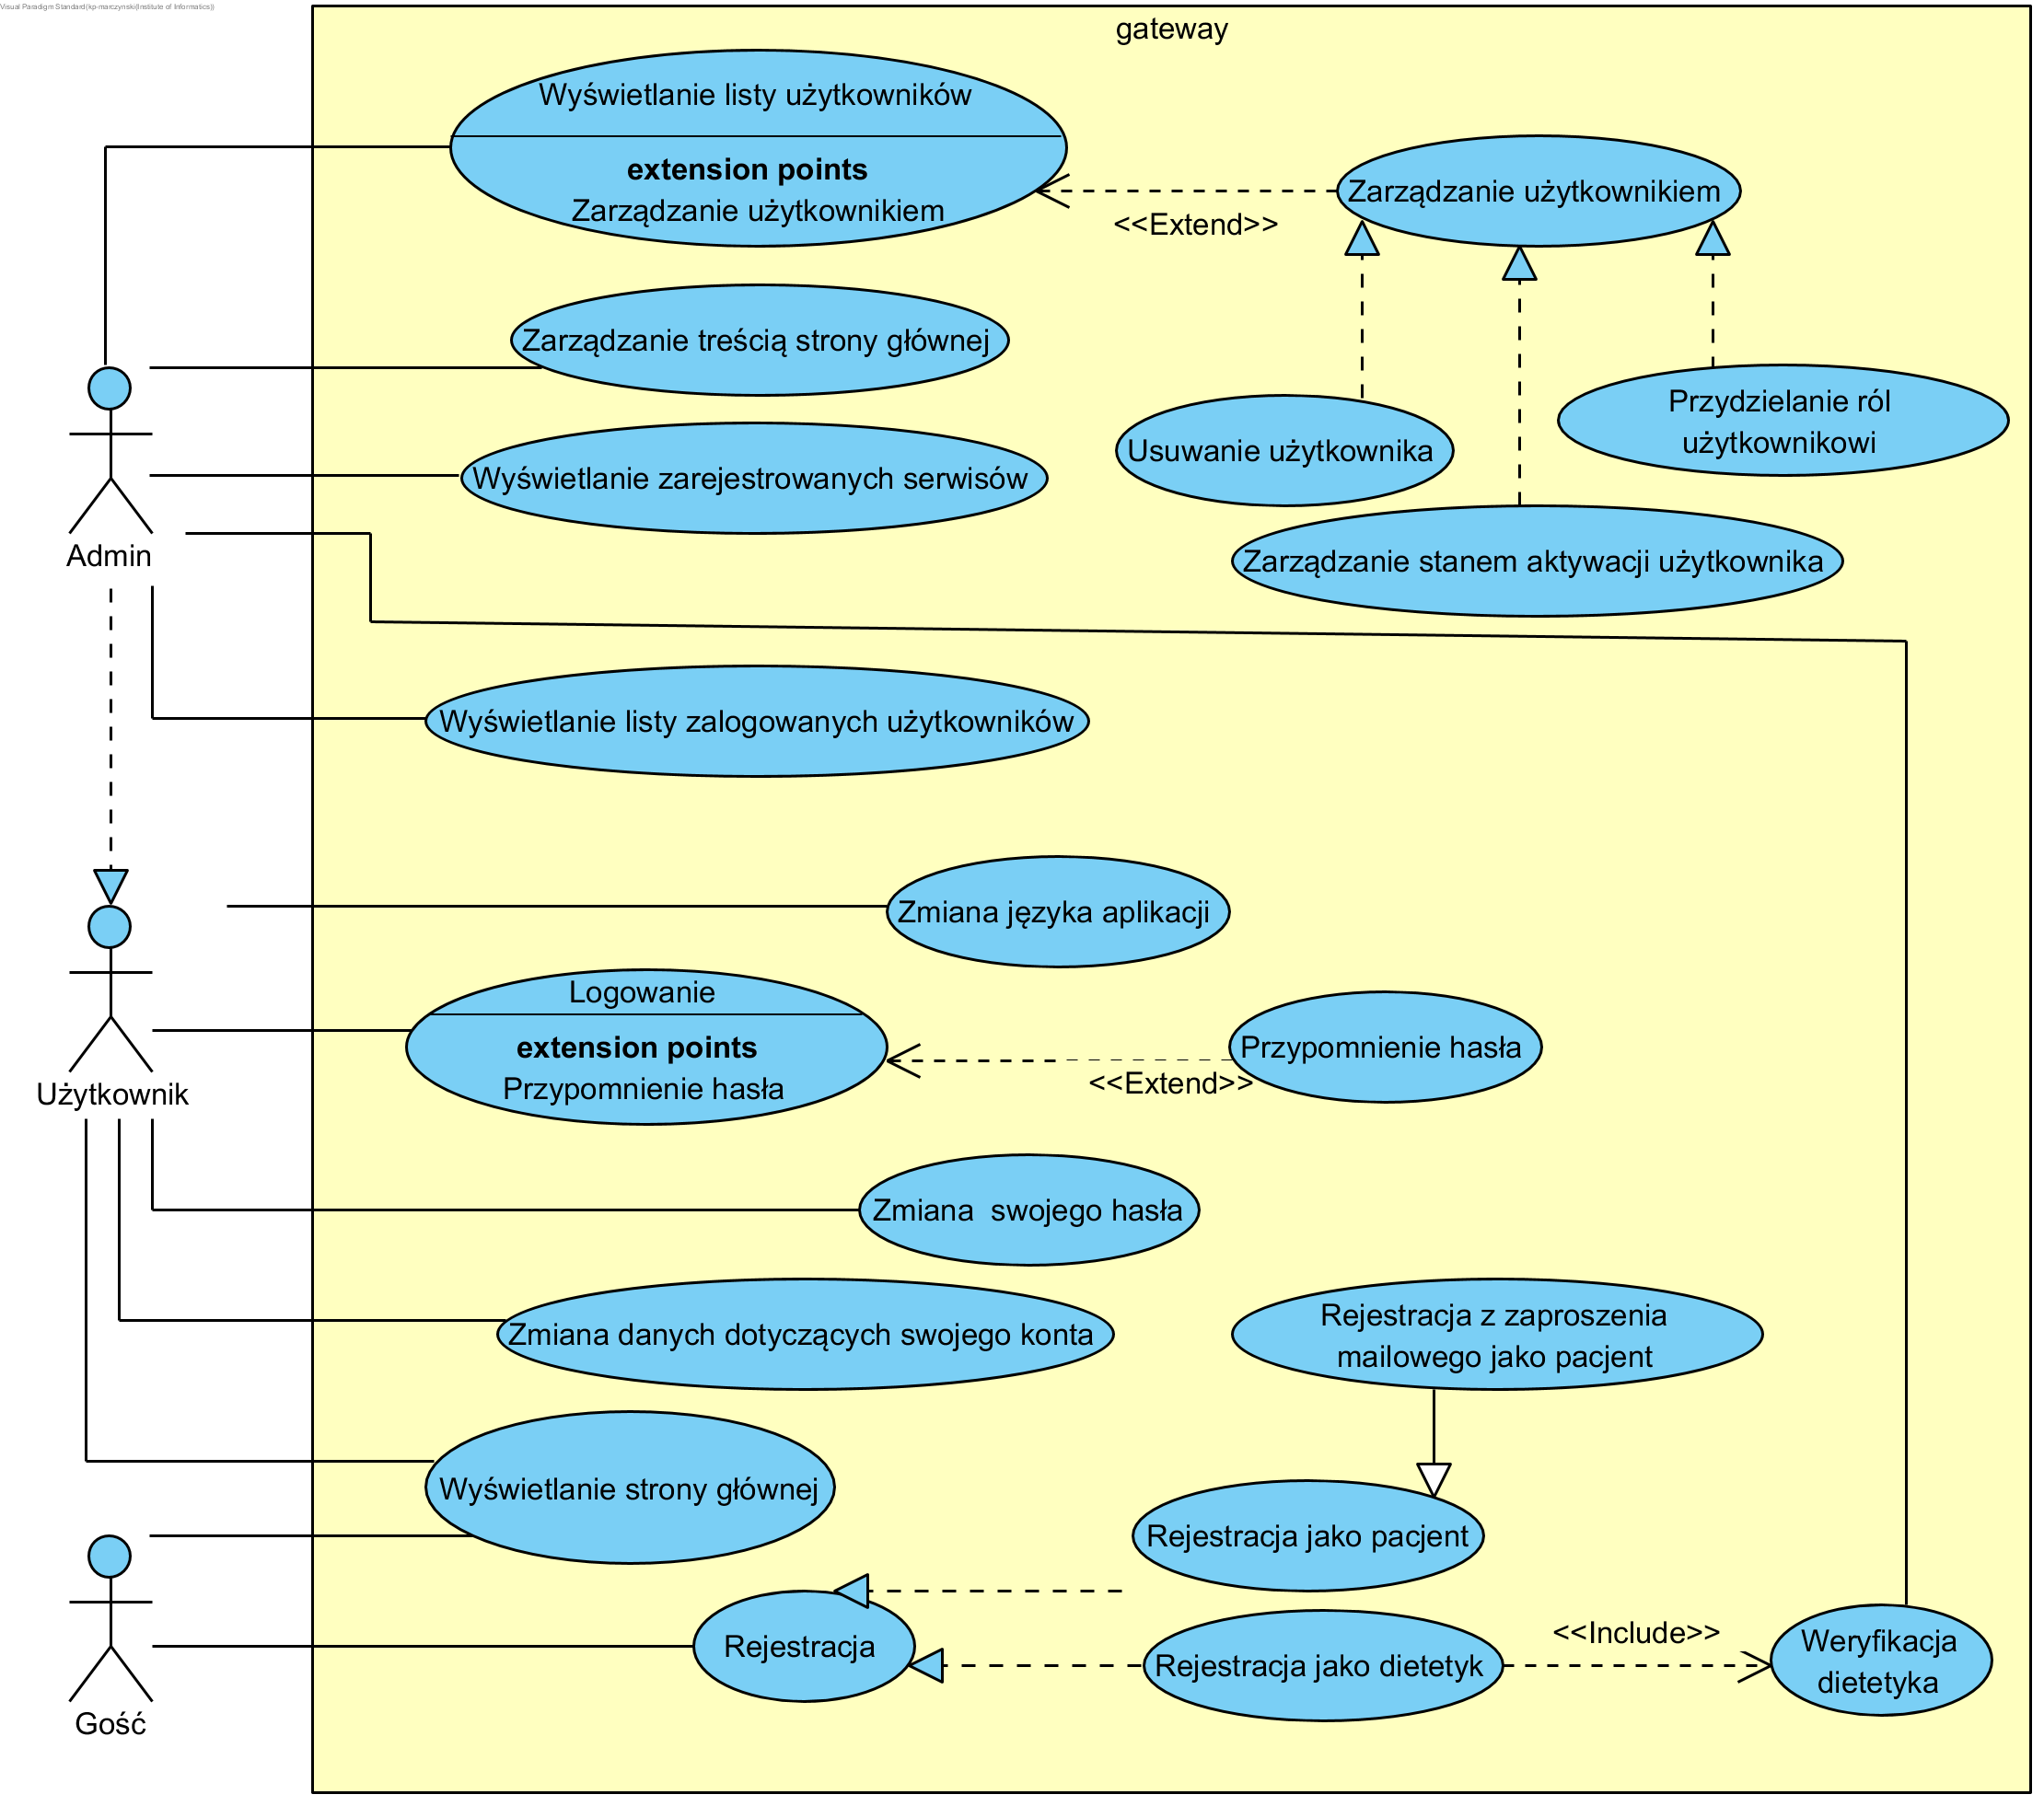
\includegraphics[scale=0.4]{../uml/use_case_diagrams/gateway.png}
        \caption{Gateway (opr.wł).}\label{rysunek:use-case-diagram-gateway}
    \end{figure}
\end{minipage}

\begin{minipage}{\textwidth}
    \begin{figure}[H]
        \centering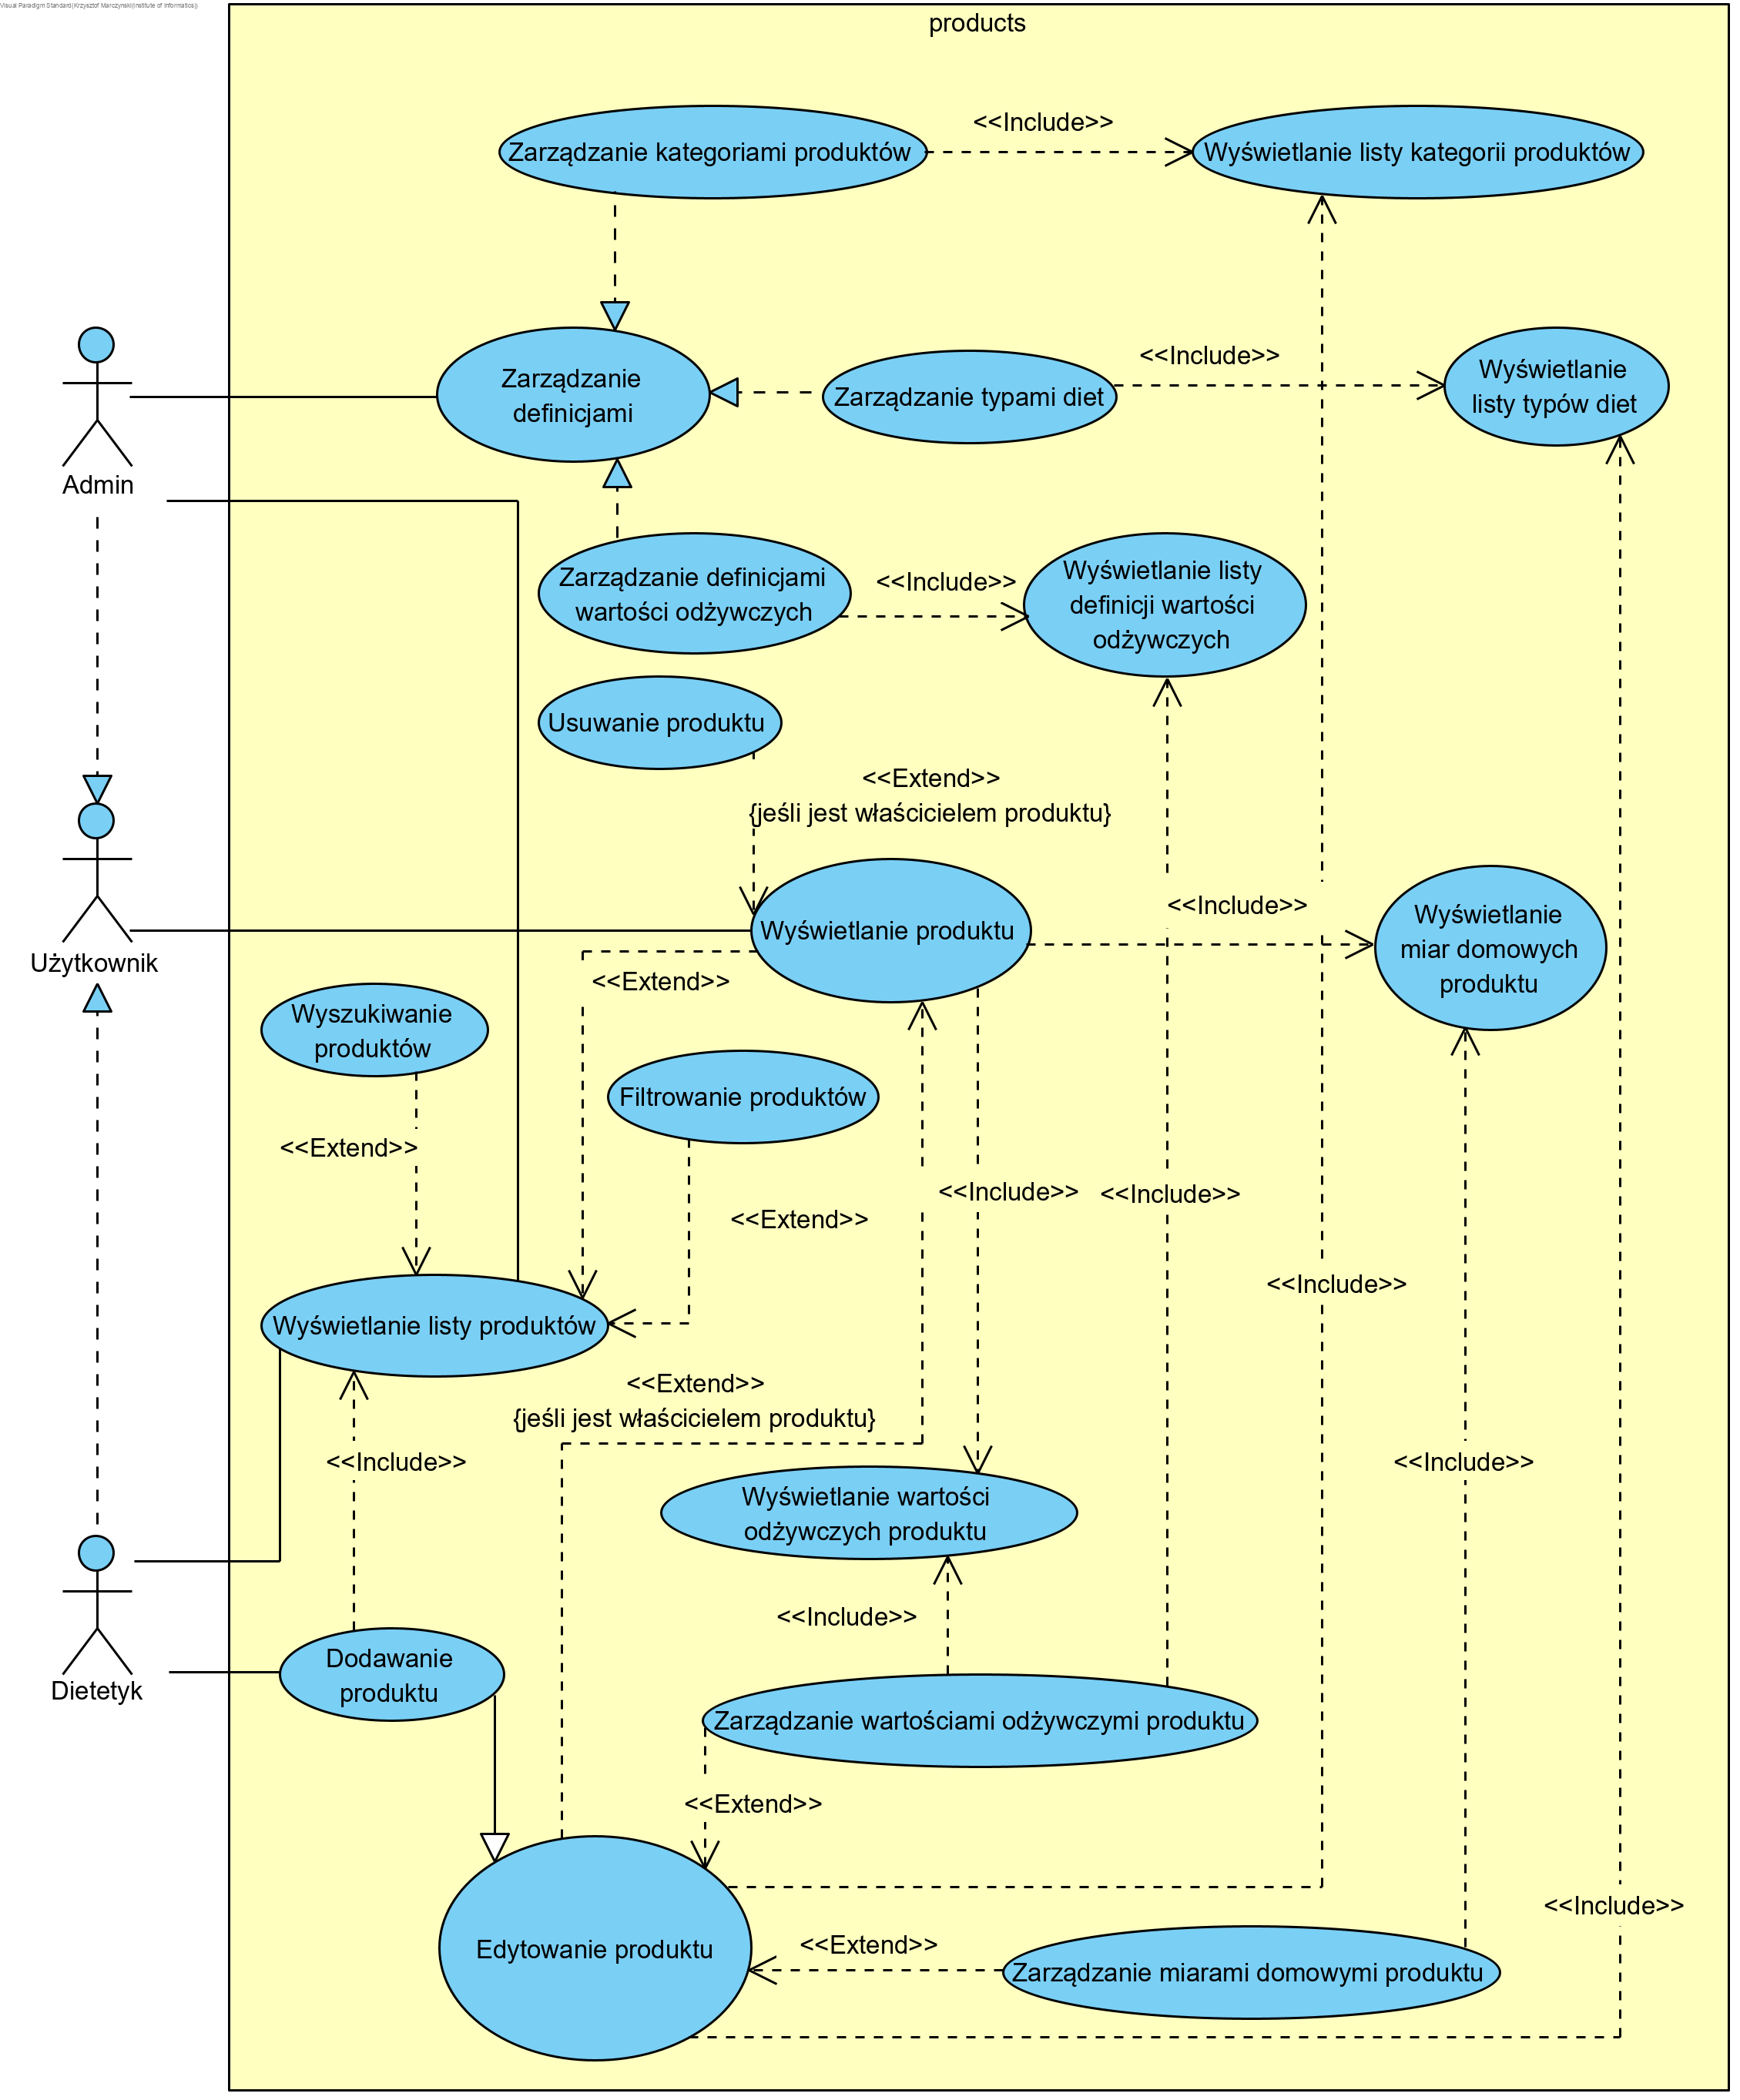
\includegraphics[scale=0.4]{../uml/use_case_diagrams/products.png}
        \caption{Produkty (opr.wł).}\label{rysunek:use-case-diagram-products}
    \end{figure}
\end{minipage}

\begin{minipage}{\textwidth}
    \begin{figure}[H]
        \centering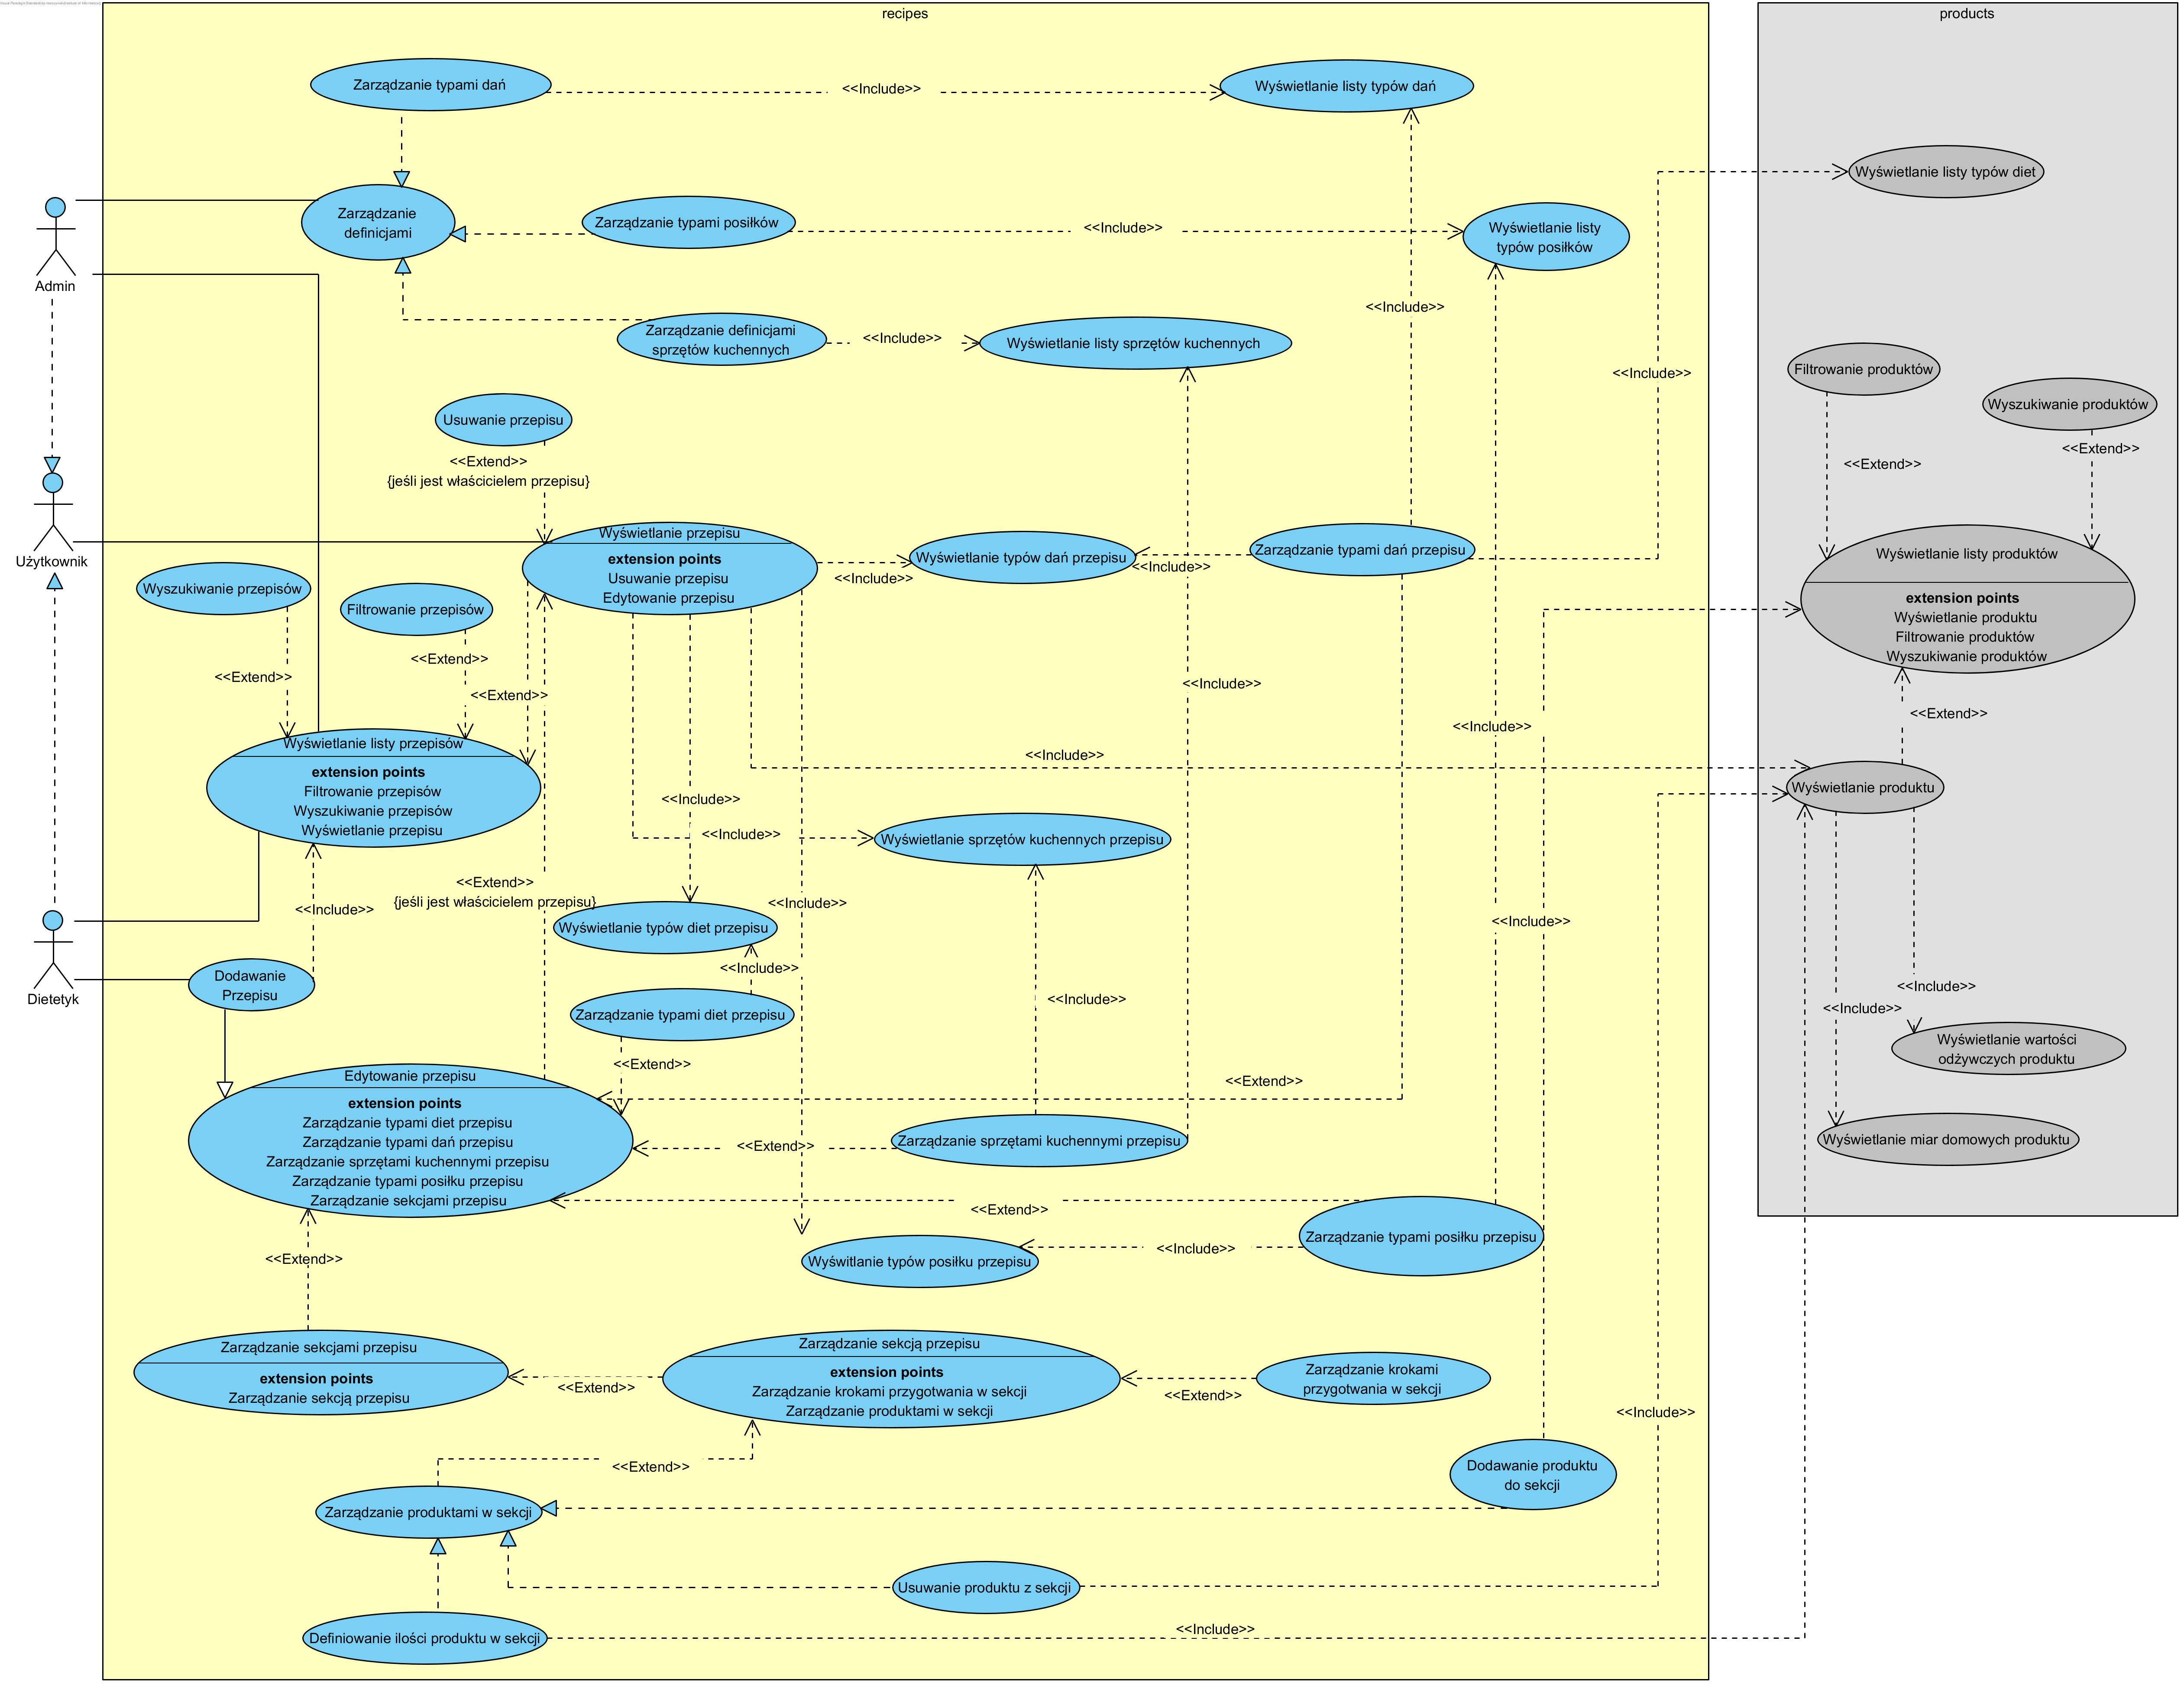
\includegraphics[scale=0.4]{../uml/use_case_diagrams/recipes.png}
        \caption{Przepisy (opr.wł).}\label{rysunek:use-case-diagram-recipes}
    \end{figure}
\end{minipage}

\begin{minipage}{\textwidth}
    \begin{figure}[H]
        \centering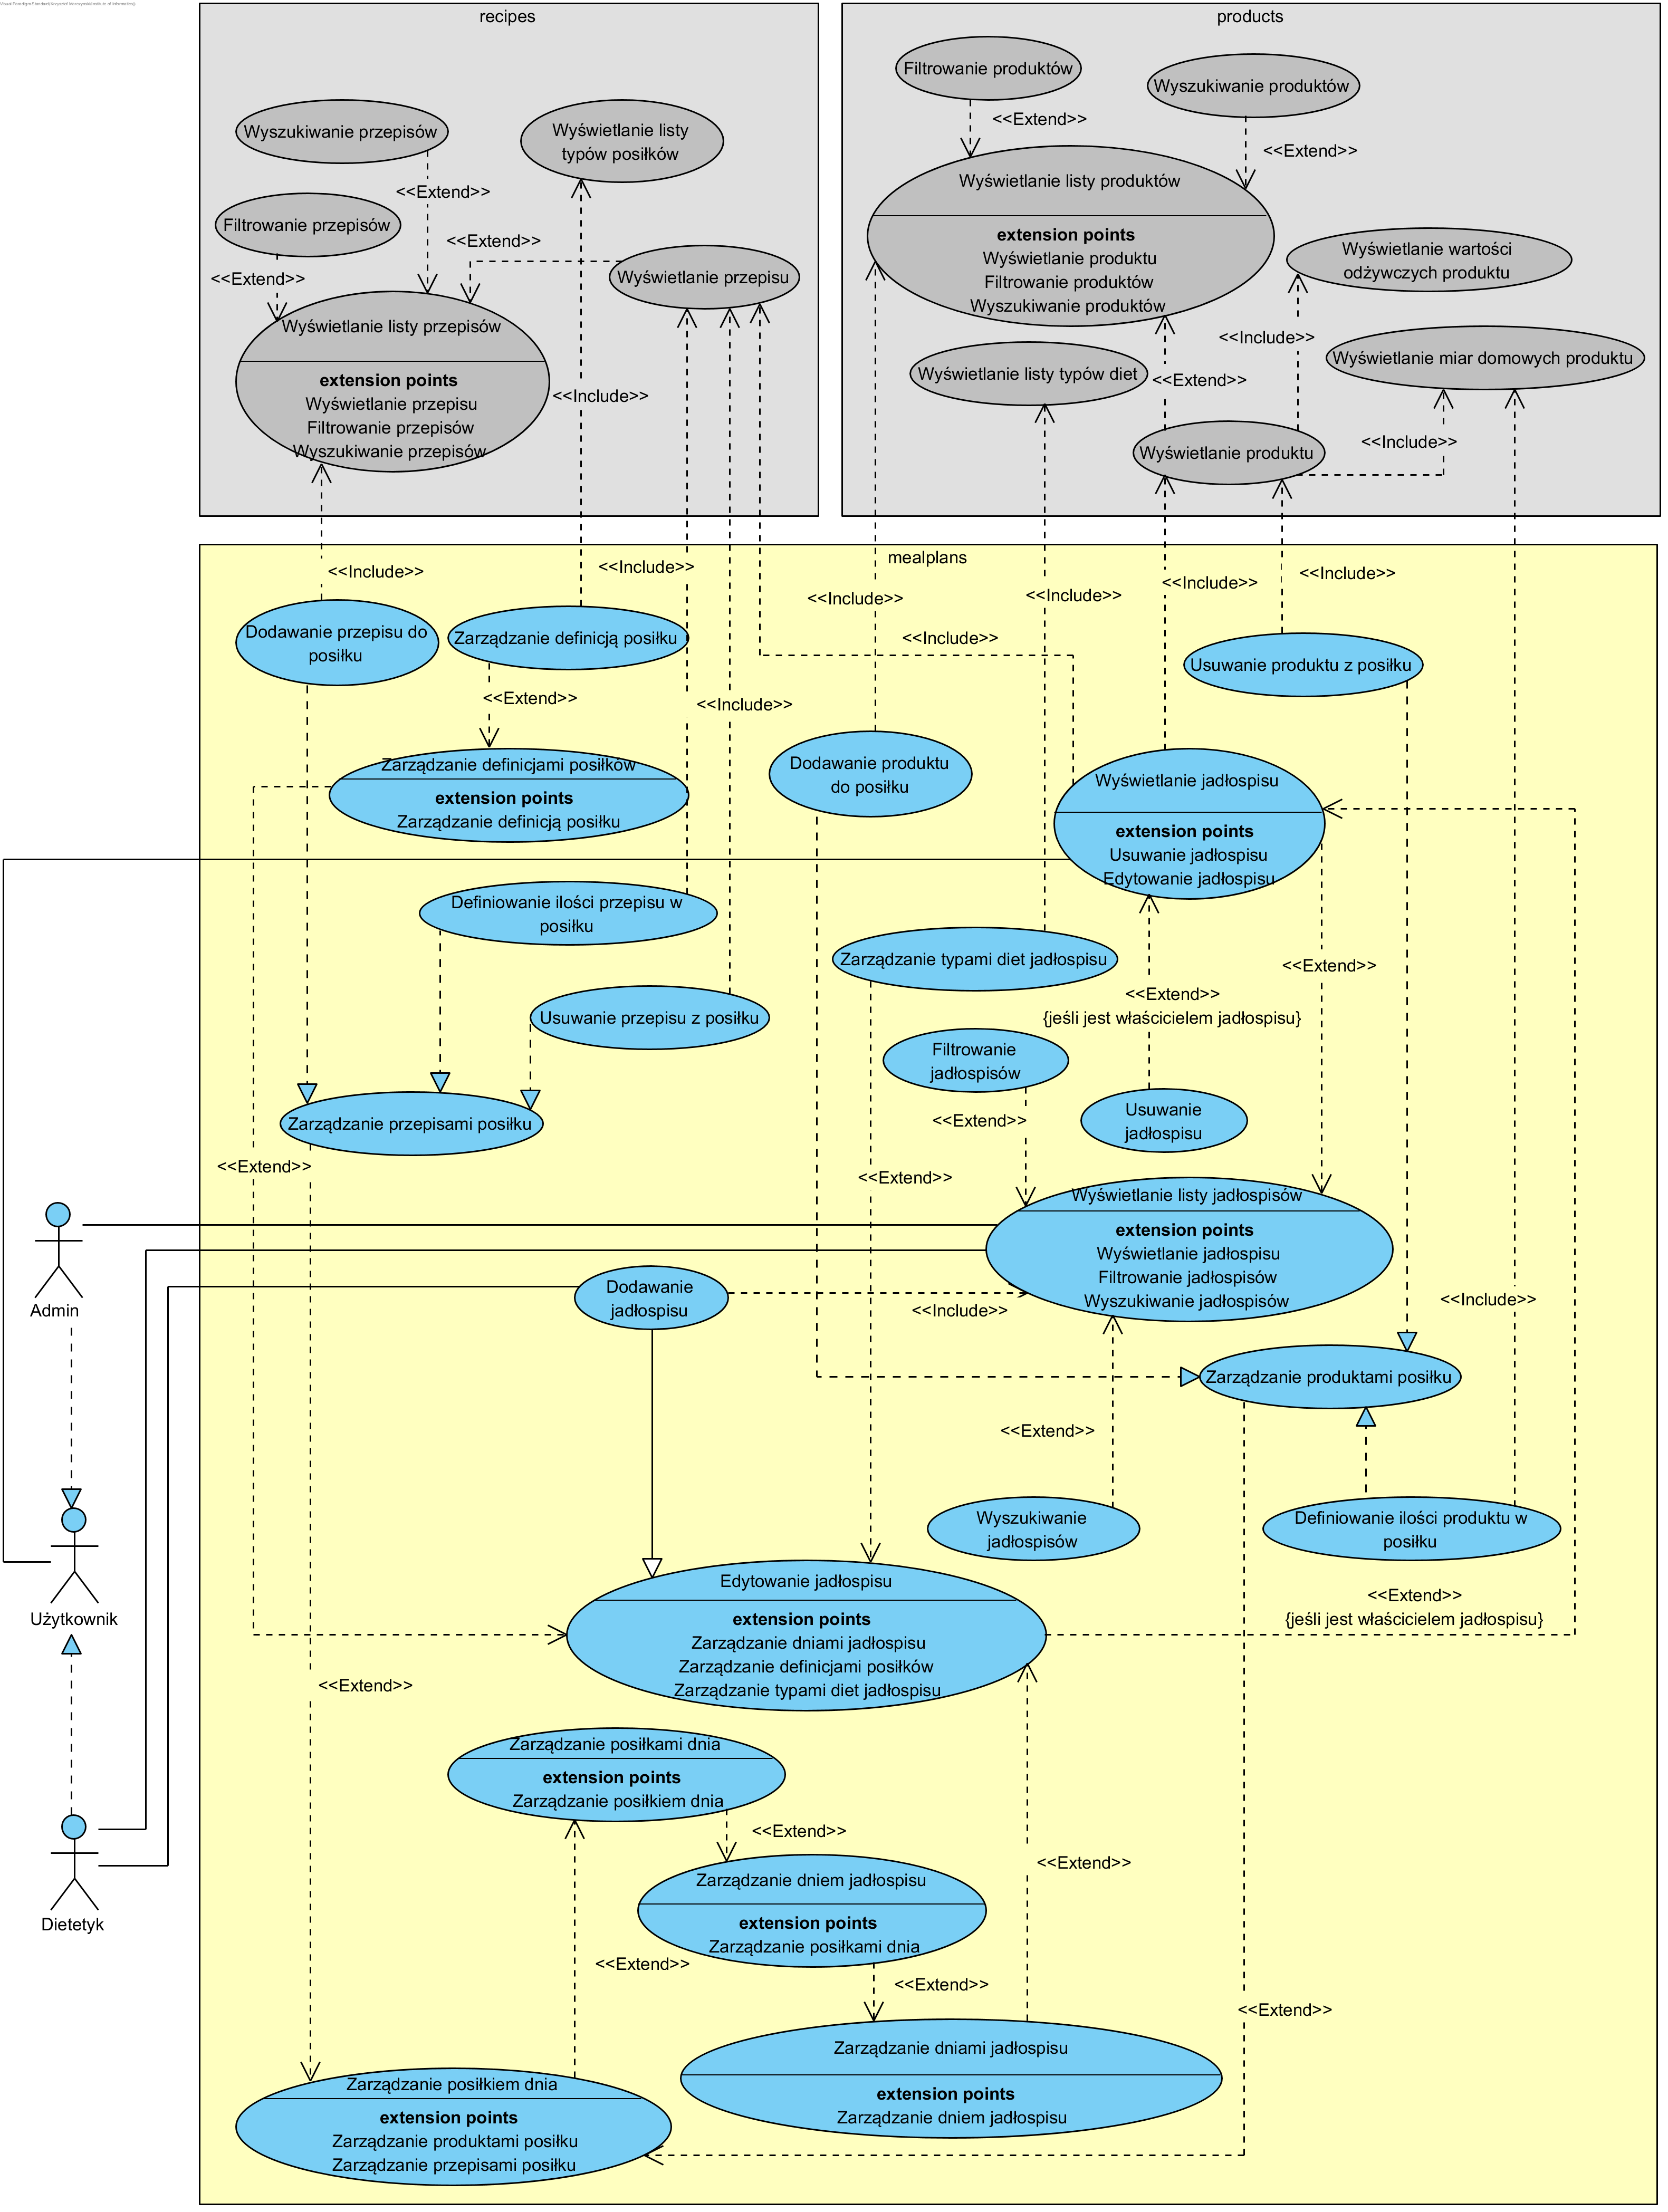
\includegraphics[scale=0.4]{../uml/use_case_diagrams/mealplans.png}
        \caption{Jadłospisy (opr.wł).}\label{rysunek:use-case-diagram-mealplans}
    \end{figure}
\end{minipage}

\begin{minipage}{\textwidth}
    \begin{figure}[H]
        \centering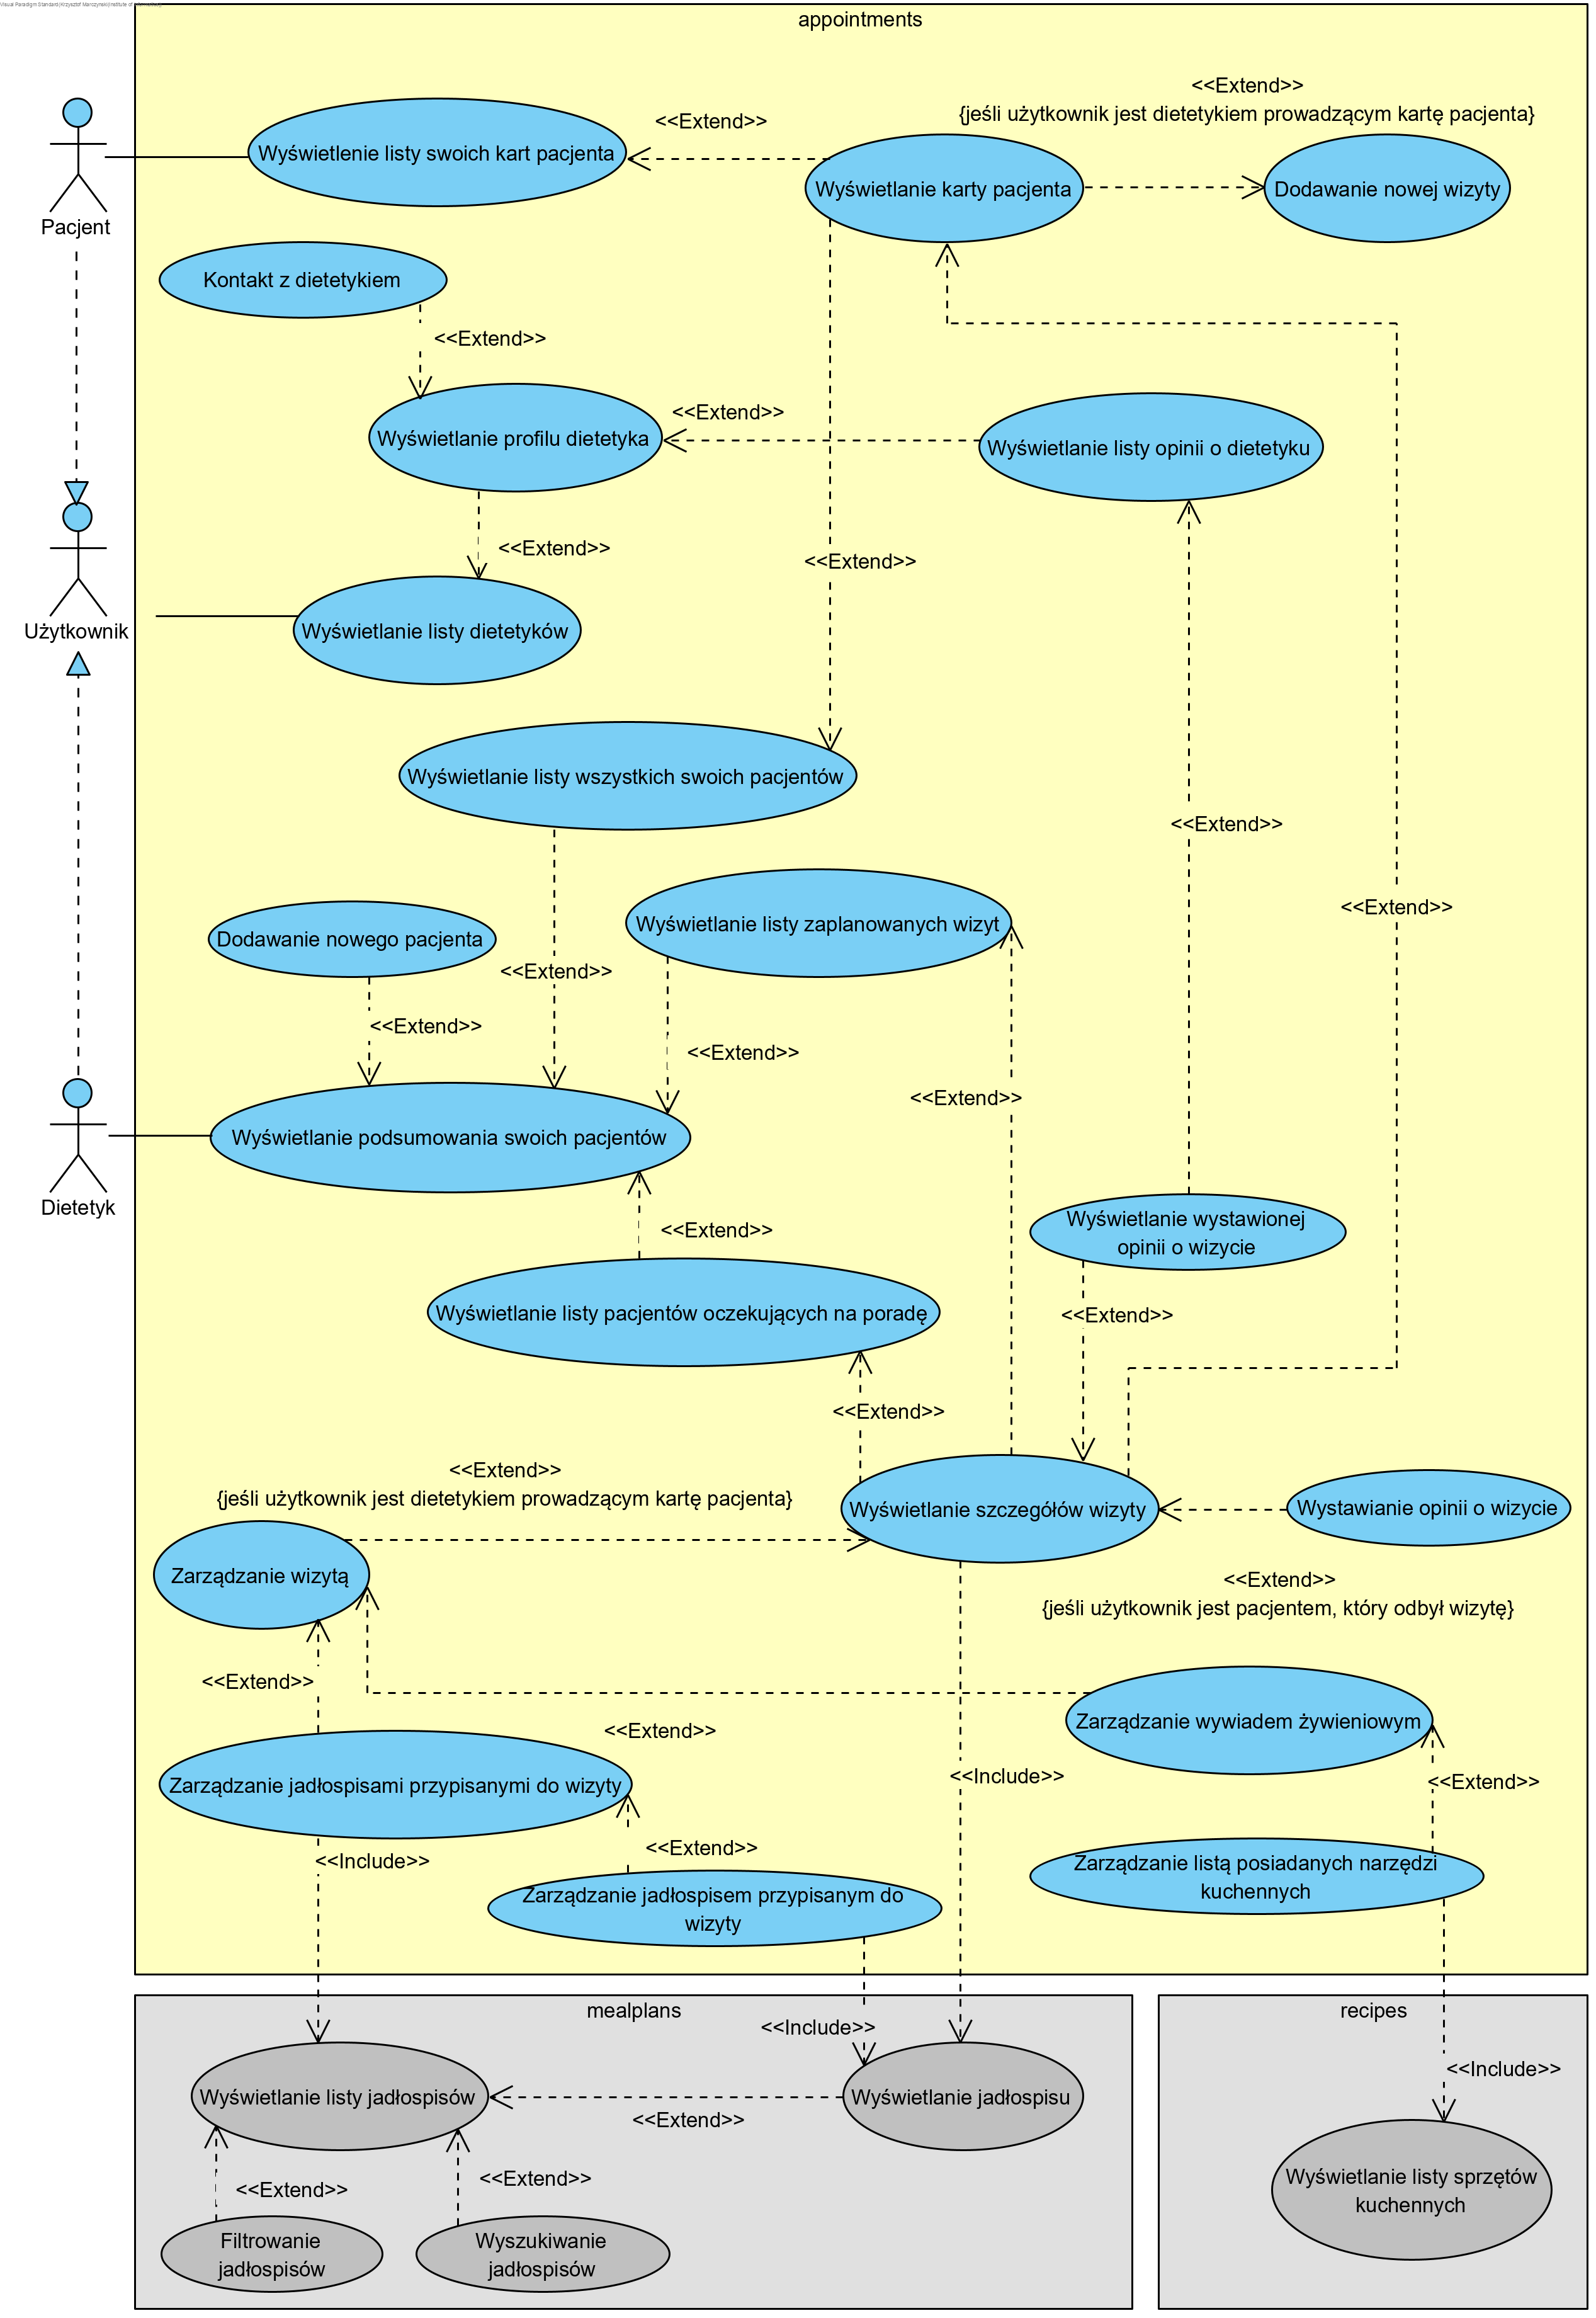
\includegraphics[scale=0.4]{../uml/use_case_diagrams/appointments.png}
        \caption{Wizyty (opr.wł).}\label{rysunek:use-case-diagram-appointments}
    \end{figure}
\end{minipage}

\section{Kategorie}
\todo{uzupełnić kategorie}

\begin{enumerate}[label={\textbf{KAT/\protect\threedigits{\theenumi}}}, wide, labelwidth=!, labelindent=0pt]
    \item \label{Product_Category} Product
    \item Language
    \item test22
    \item test3
\end{enumerate}

\section {Reguły funkcjonowania}
\todo{uzupełnić reguły funkcjonowania}

\begin{enumerate}[label={\textbf{REG/\protect\threedigits{\theenumi}}}, wide, labelwidth=!, labelindent=0pt]
    \subsection{Produkty}
    \item test1
    \item test2
    \subsection{Przepisy}

    \subsubsection{\ref{Product_Category} Product}
    \subsection{Jadłospisy}
    \item test22
    \item test3
\end{enumerate}

\section{Ograniczenia dziedzinowe}
\todo{uzupełnić ograniczenia dziedzionowe}
\section{Model domenowy}
\todo{diagram klas}

\begin{minipage}{\textwidth}
    \begin{figure}[H]
        \centering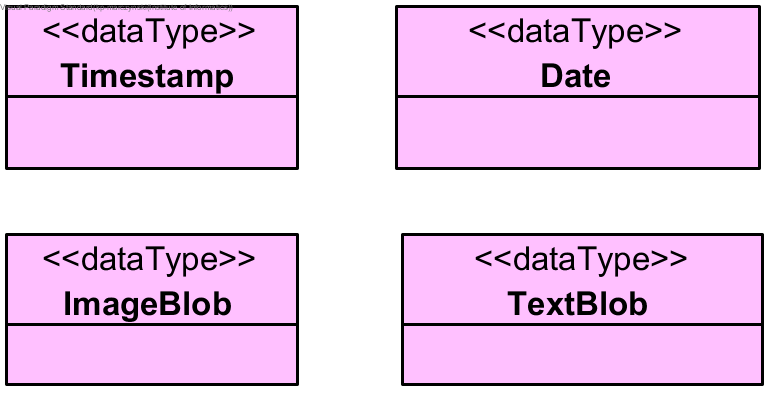
\includegraphics[scale=0.6]{../uml/class_diagrams/dataTypes.png}
        \caption{Typy danych (opr.wł).}\label{rysunek:class-diagram-data-types}
    \end{figure}
\end{minipage}

\begin{minipage}{\textwidth}
    \begin{figure}[H]
        \centering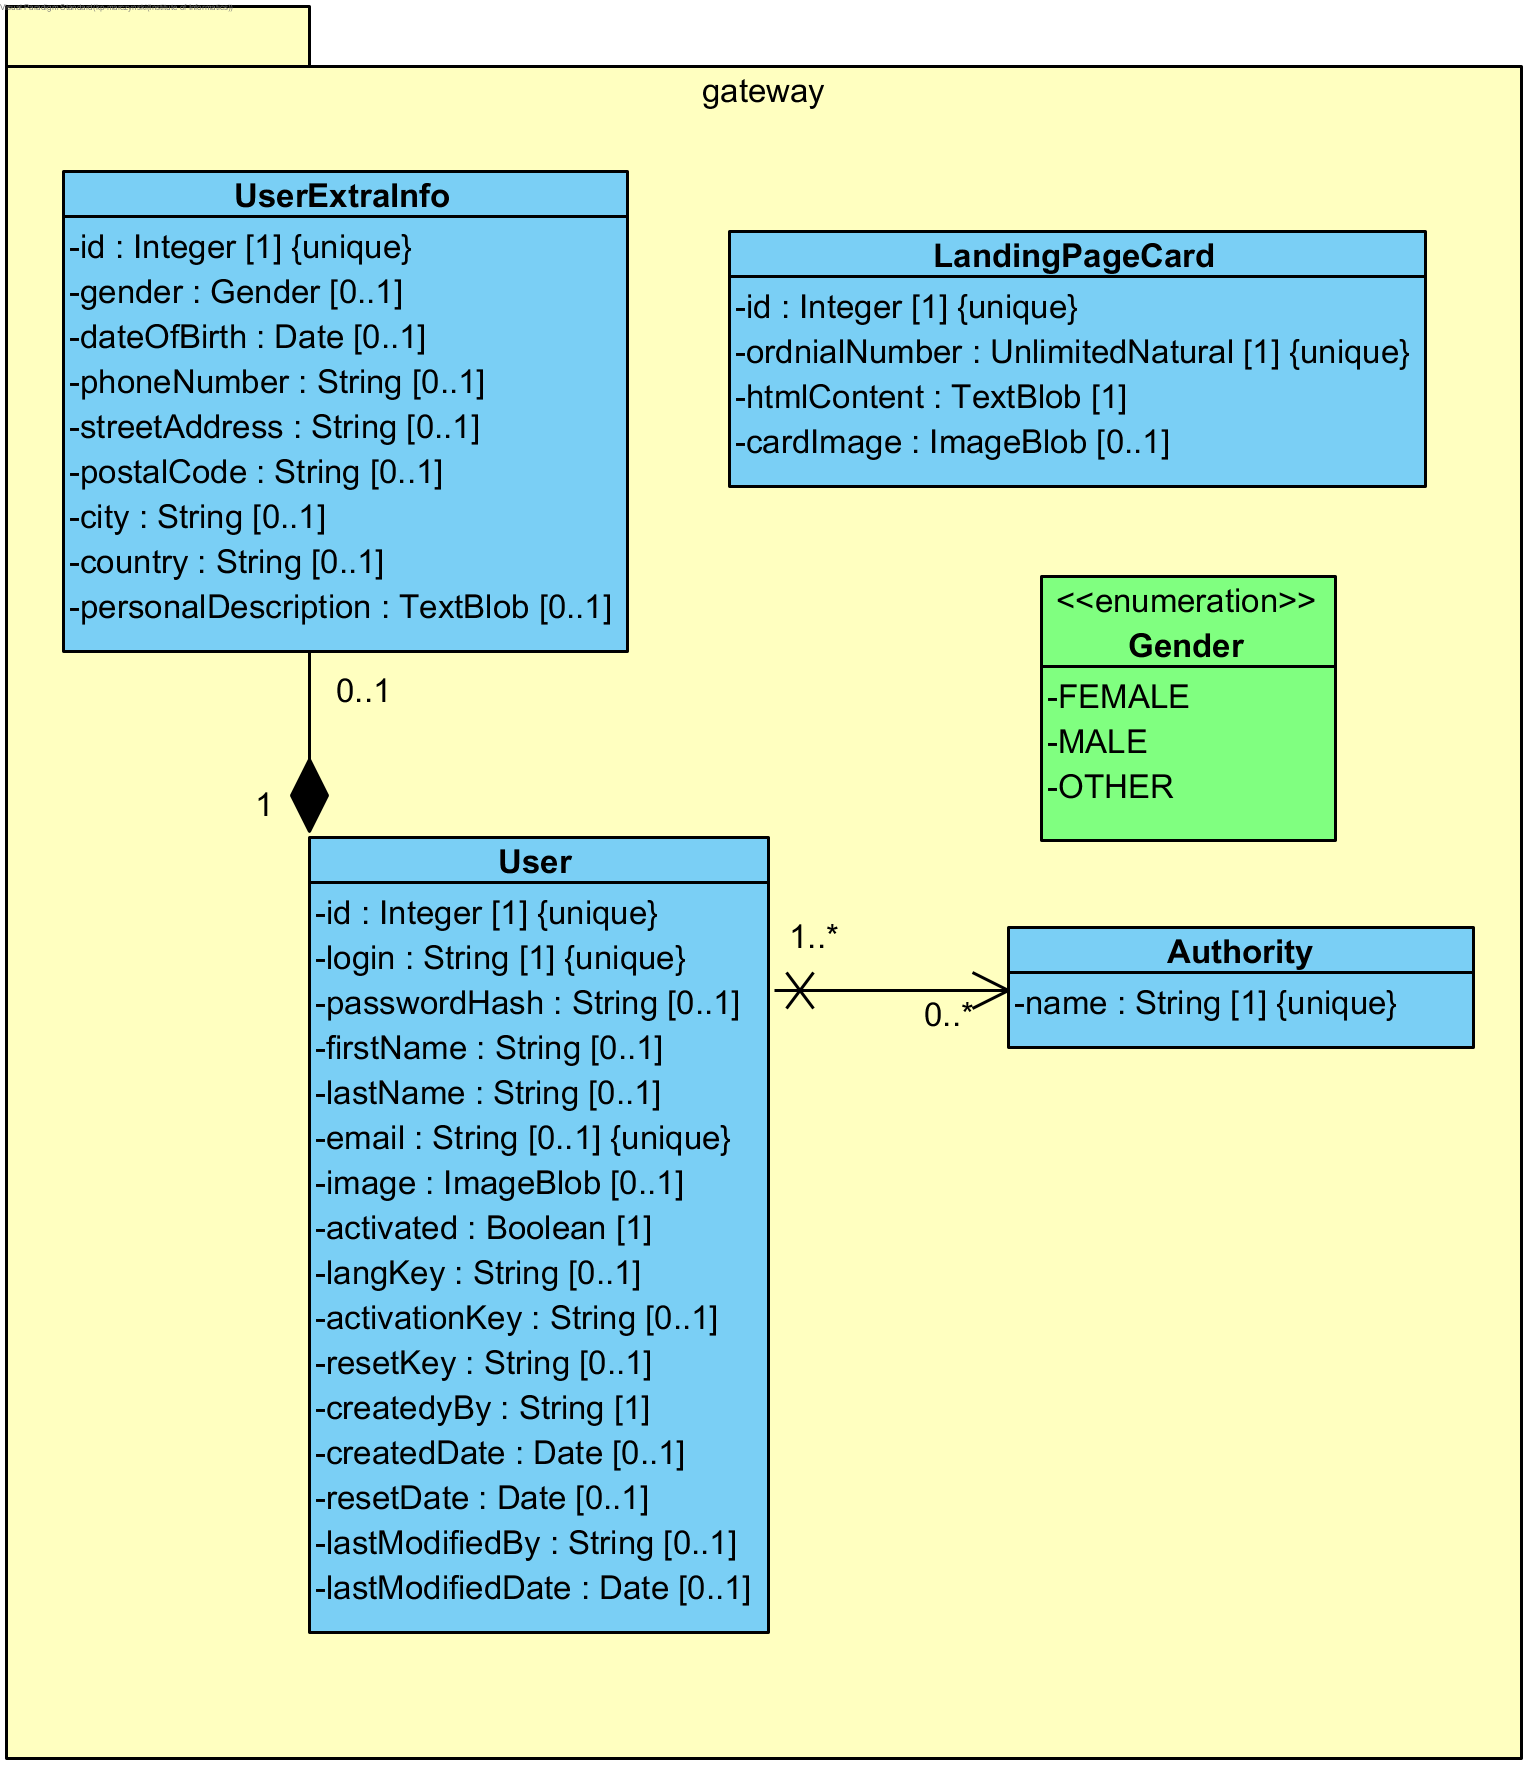
\includegraphics[scale=0.6]{../uml/class_diagrams/gateway.png}
        \caption{Gateway (opr.wł).}\label{rysunek:class-diagram-gateway}
    \end{figure}
\end{minipage}

\begin{minipage}{\textwidth}
    \begin{figure}[H]
        \centering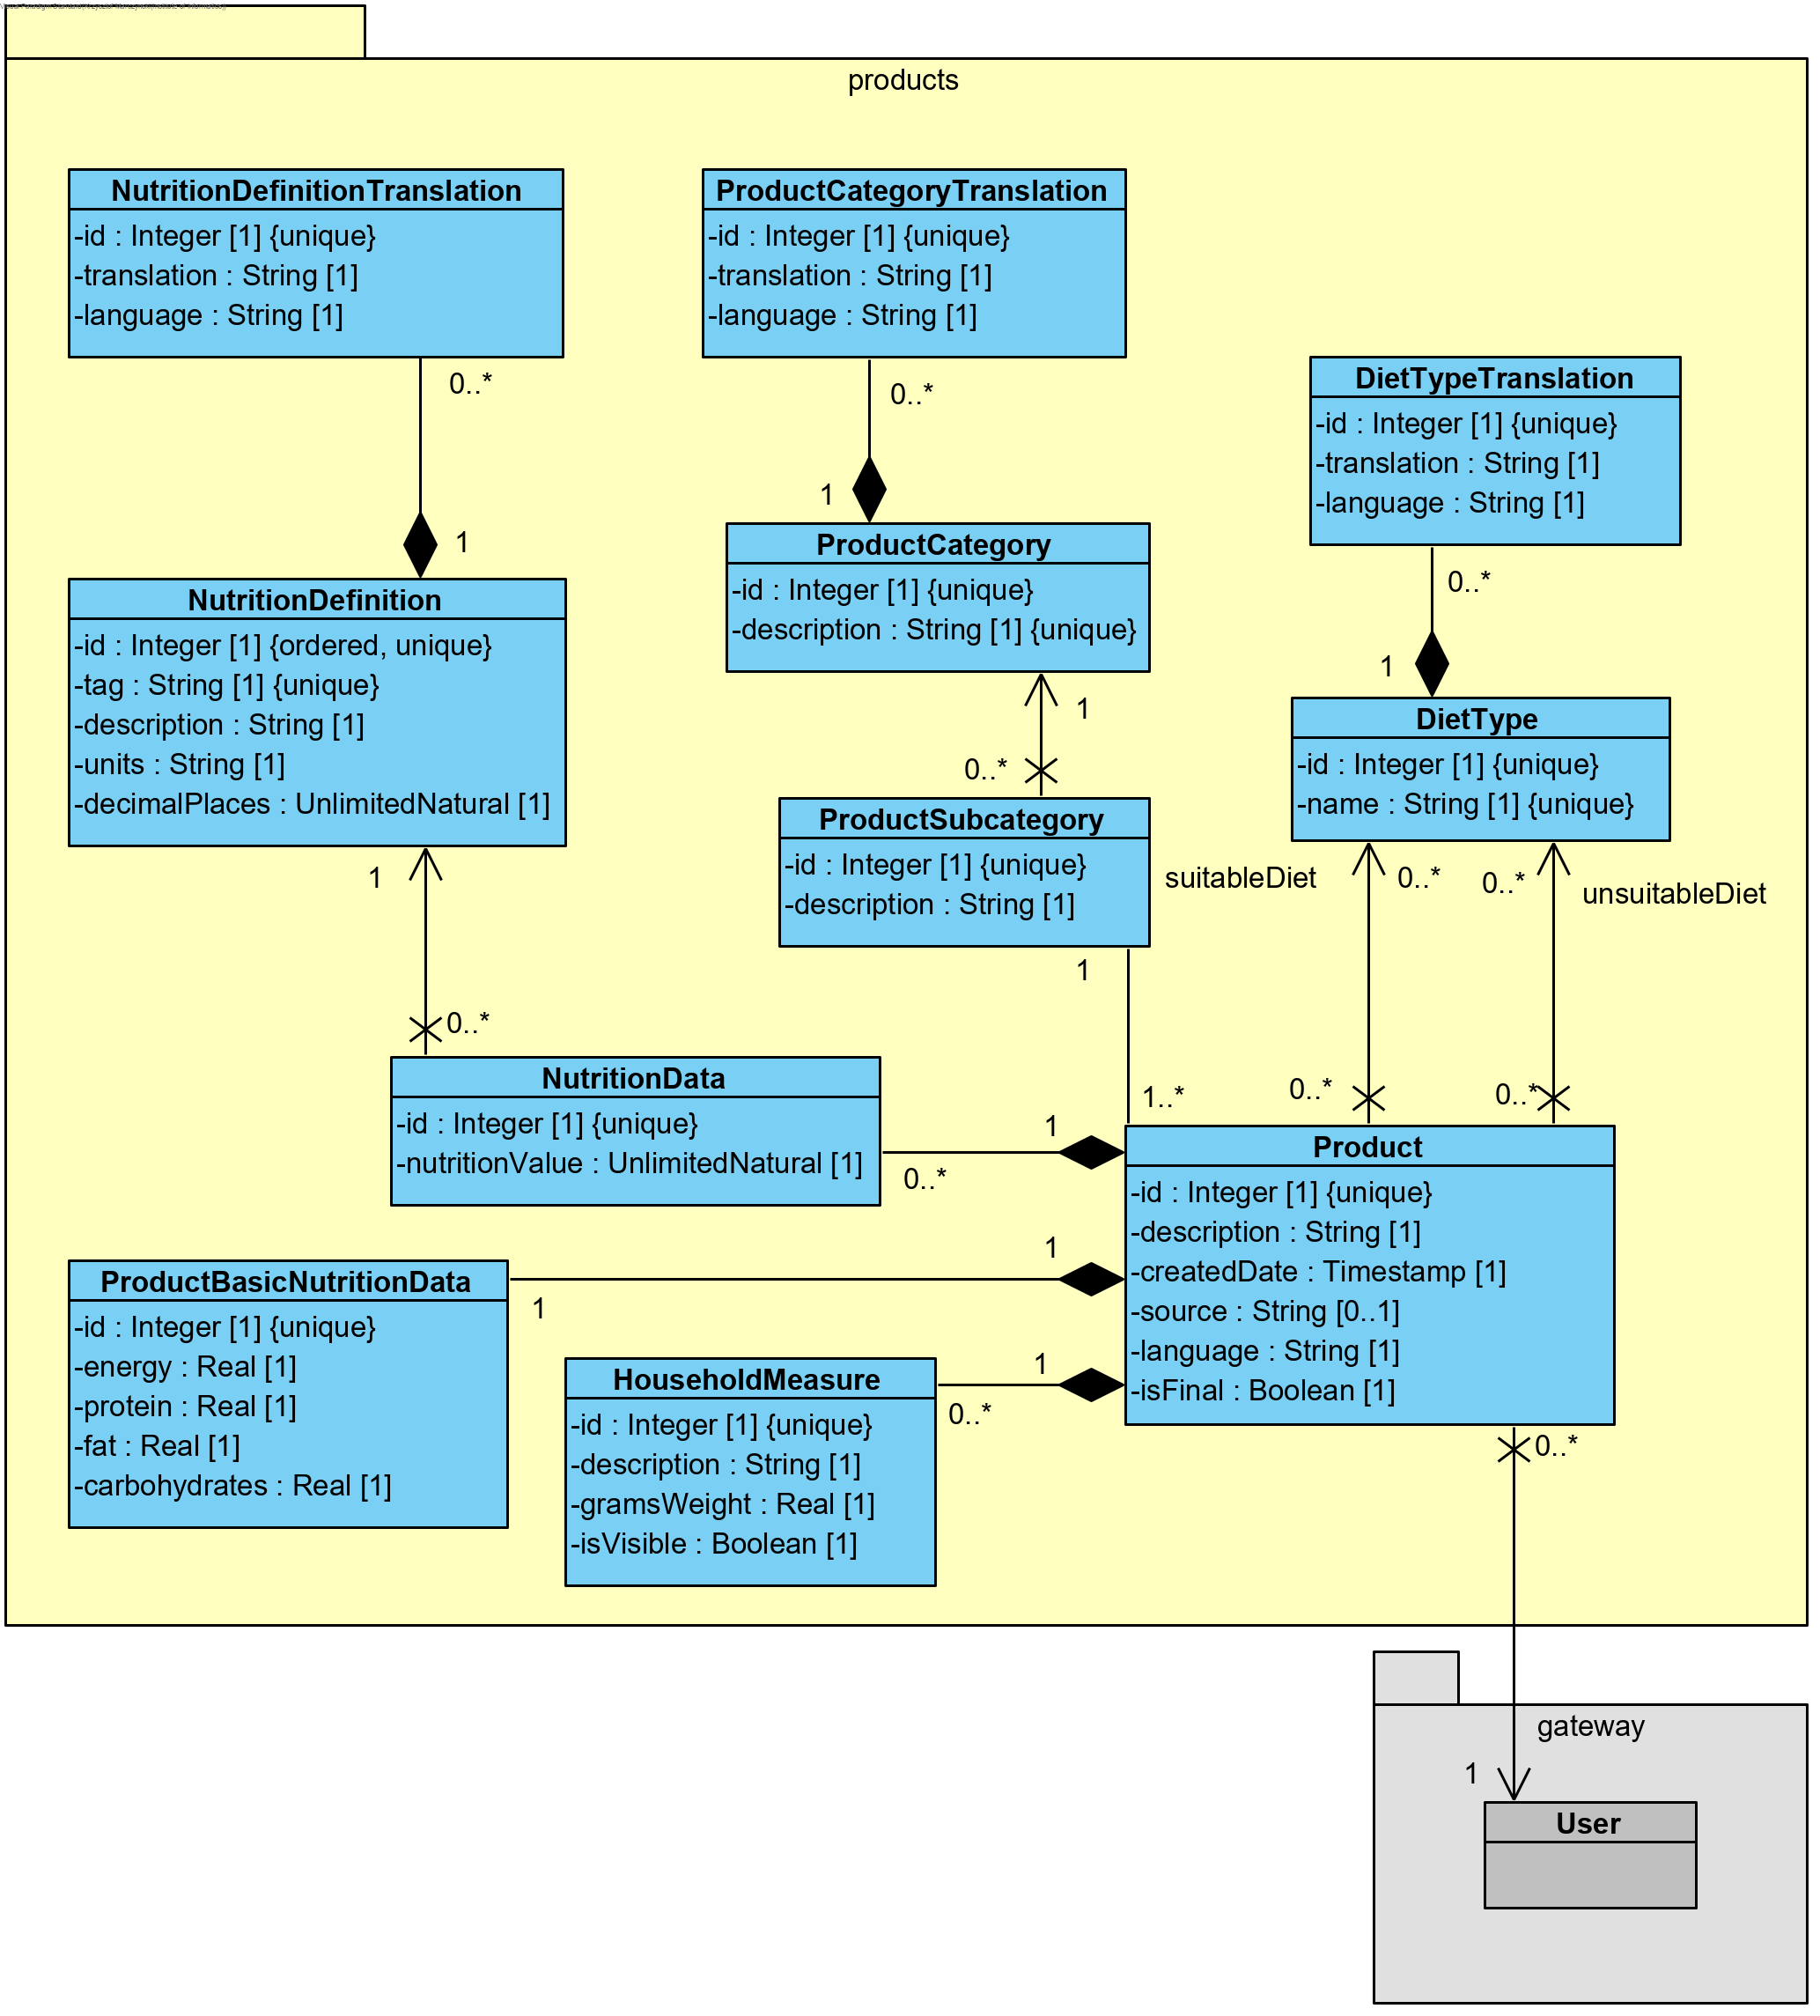
\includegraphics[scale=0.6]{../uml/class_diagrams/products.png}
        \caption{Produkty (opr.wł).}\label{rysunek:class-diagram-products}
    \end{figure}
\end{minipage}

\begin{minipage}{\textwidth}
    \begin{figure}[H]
        \centering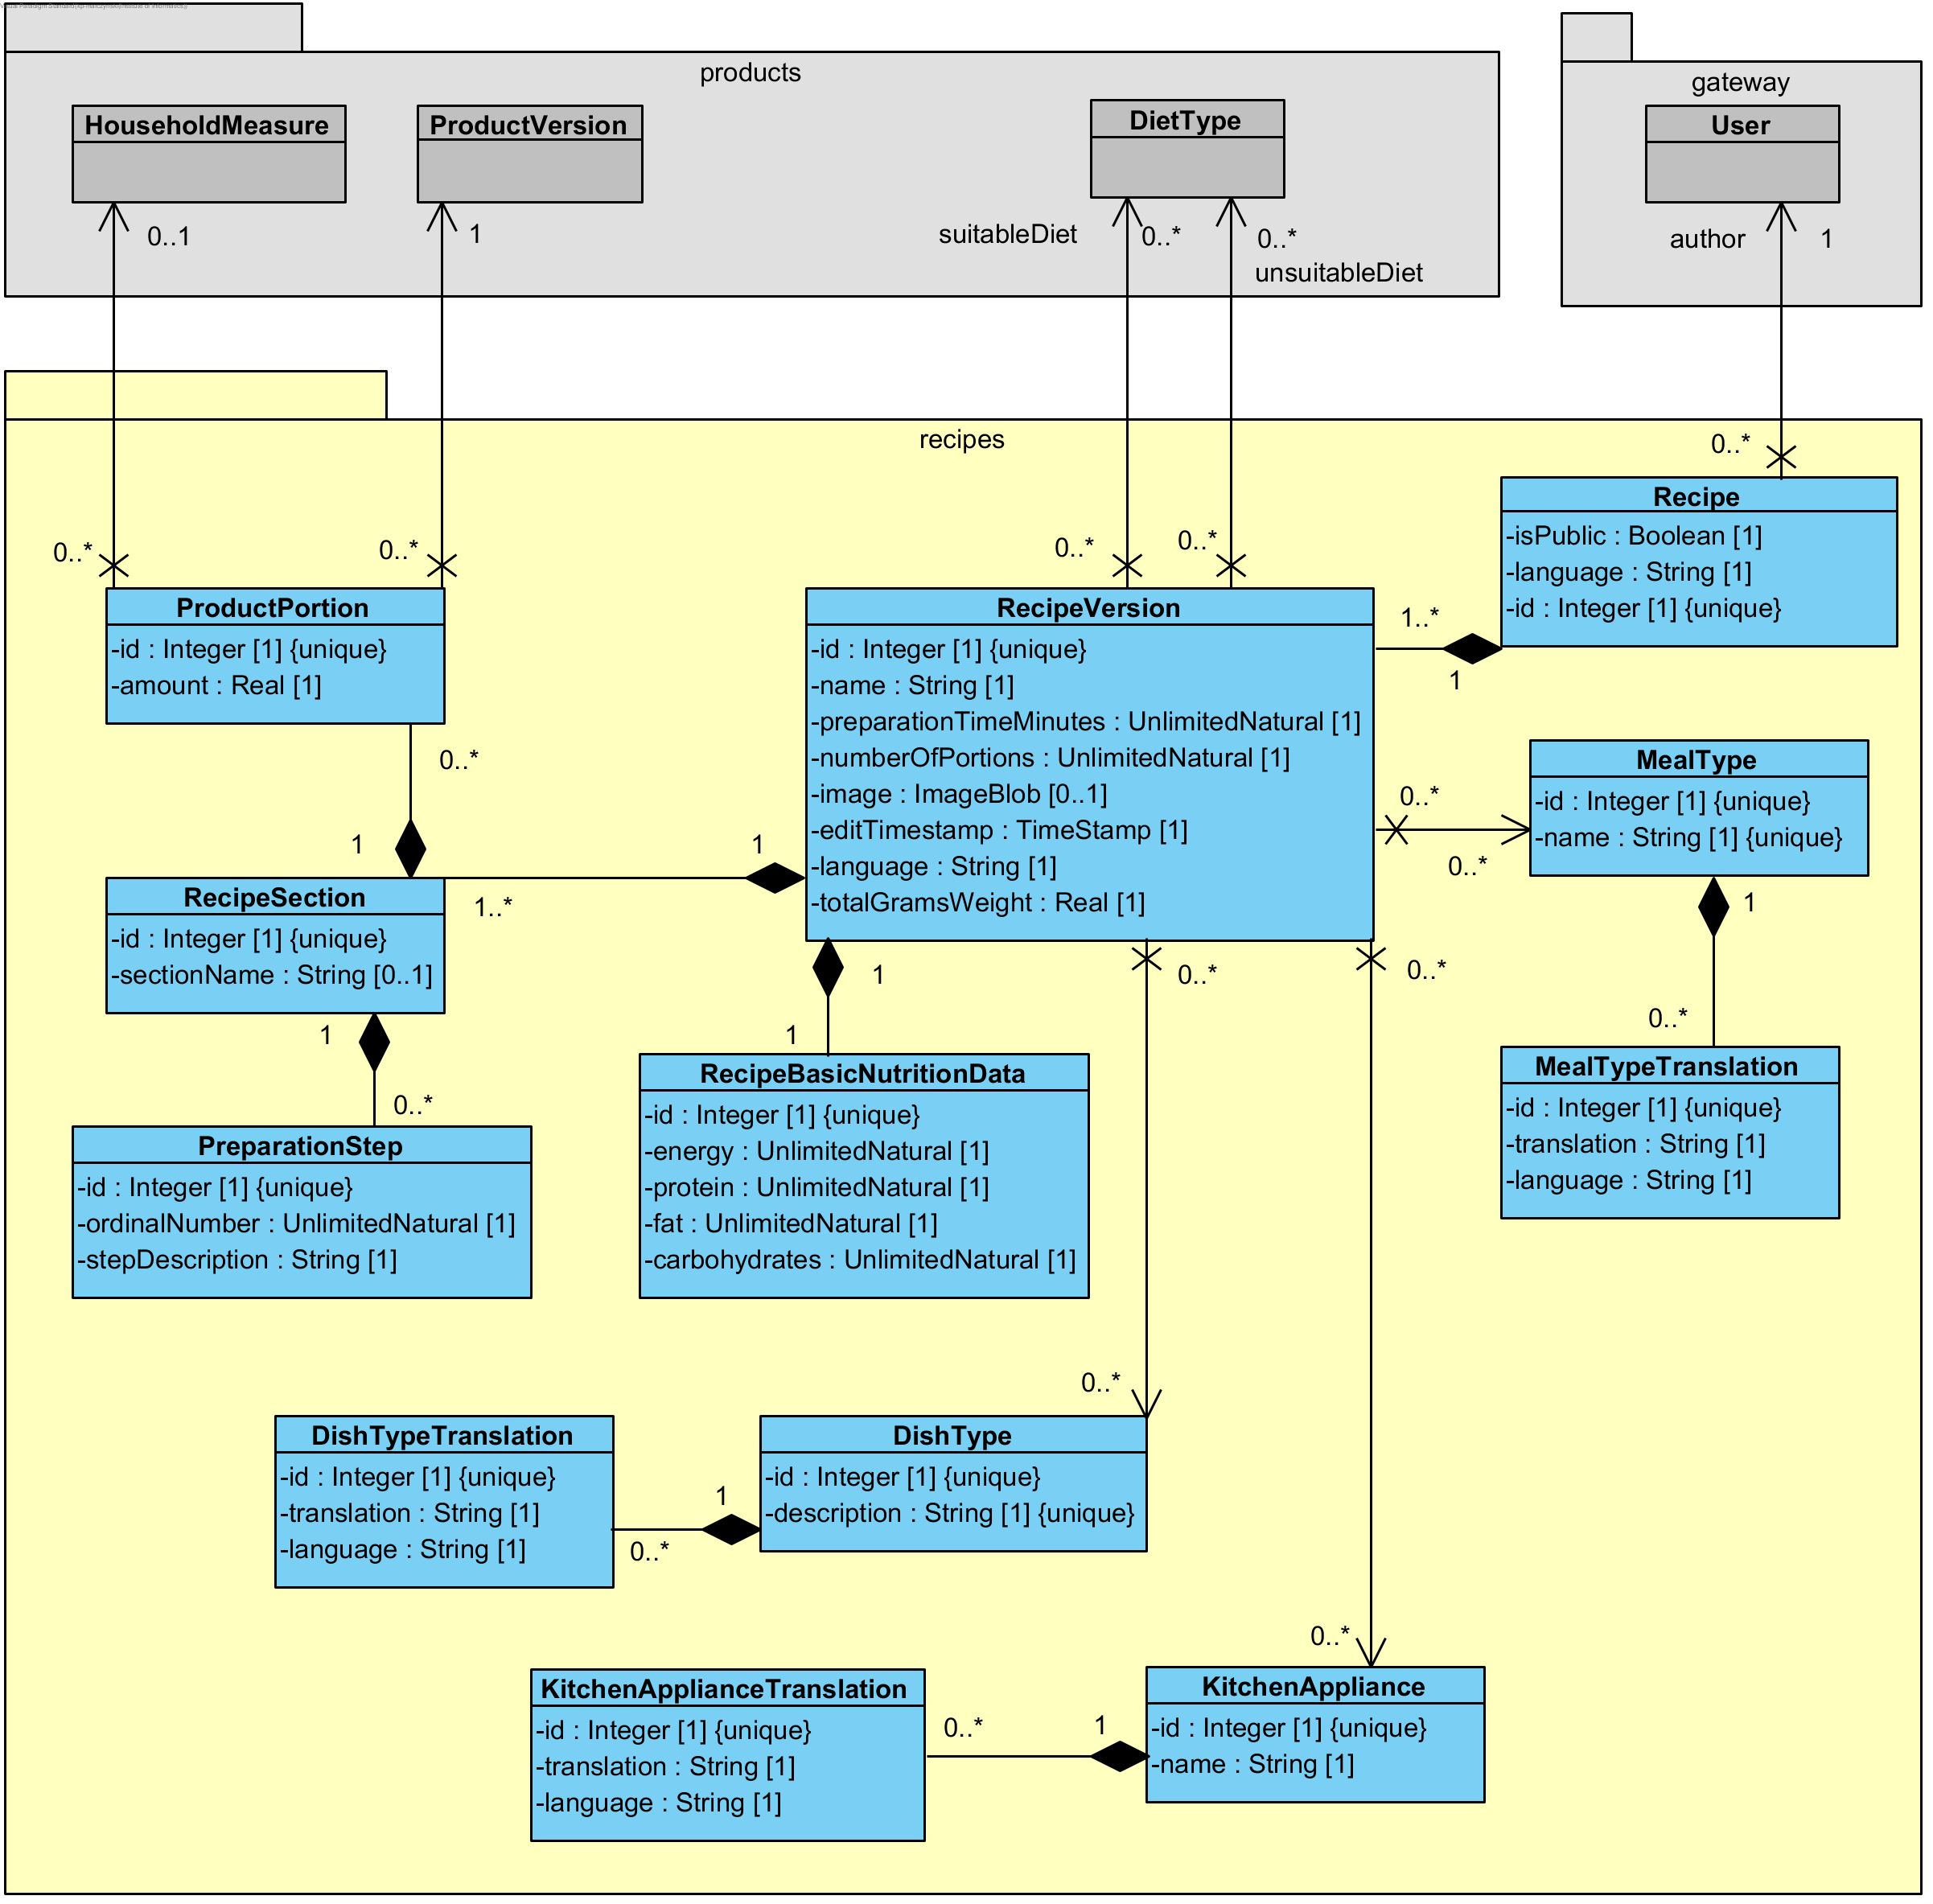
\includegraphics[scale=0.6]{../uml/class_diagrams/recipes.png}
        \caption{Przepisy (opr.wł).}\label{rysunek:class-diagram-recipes}
    \end{figure}
\end{minipage}

\begin{minipage}{\textwidth}
    \begin{figure}[H]
        \centering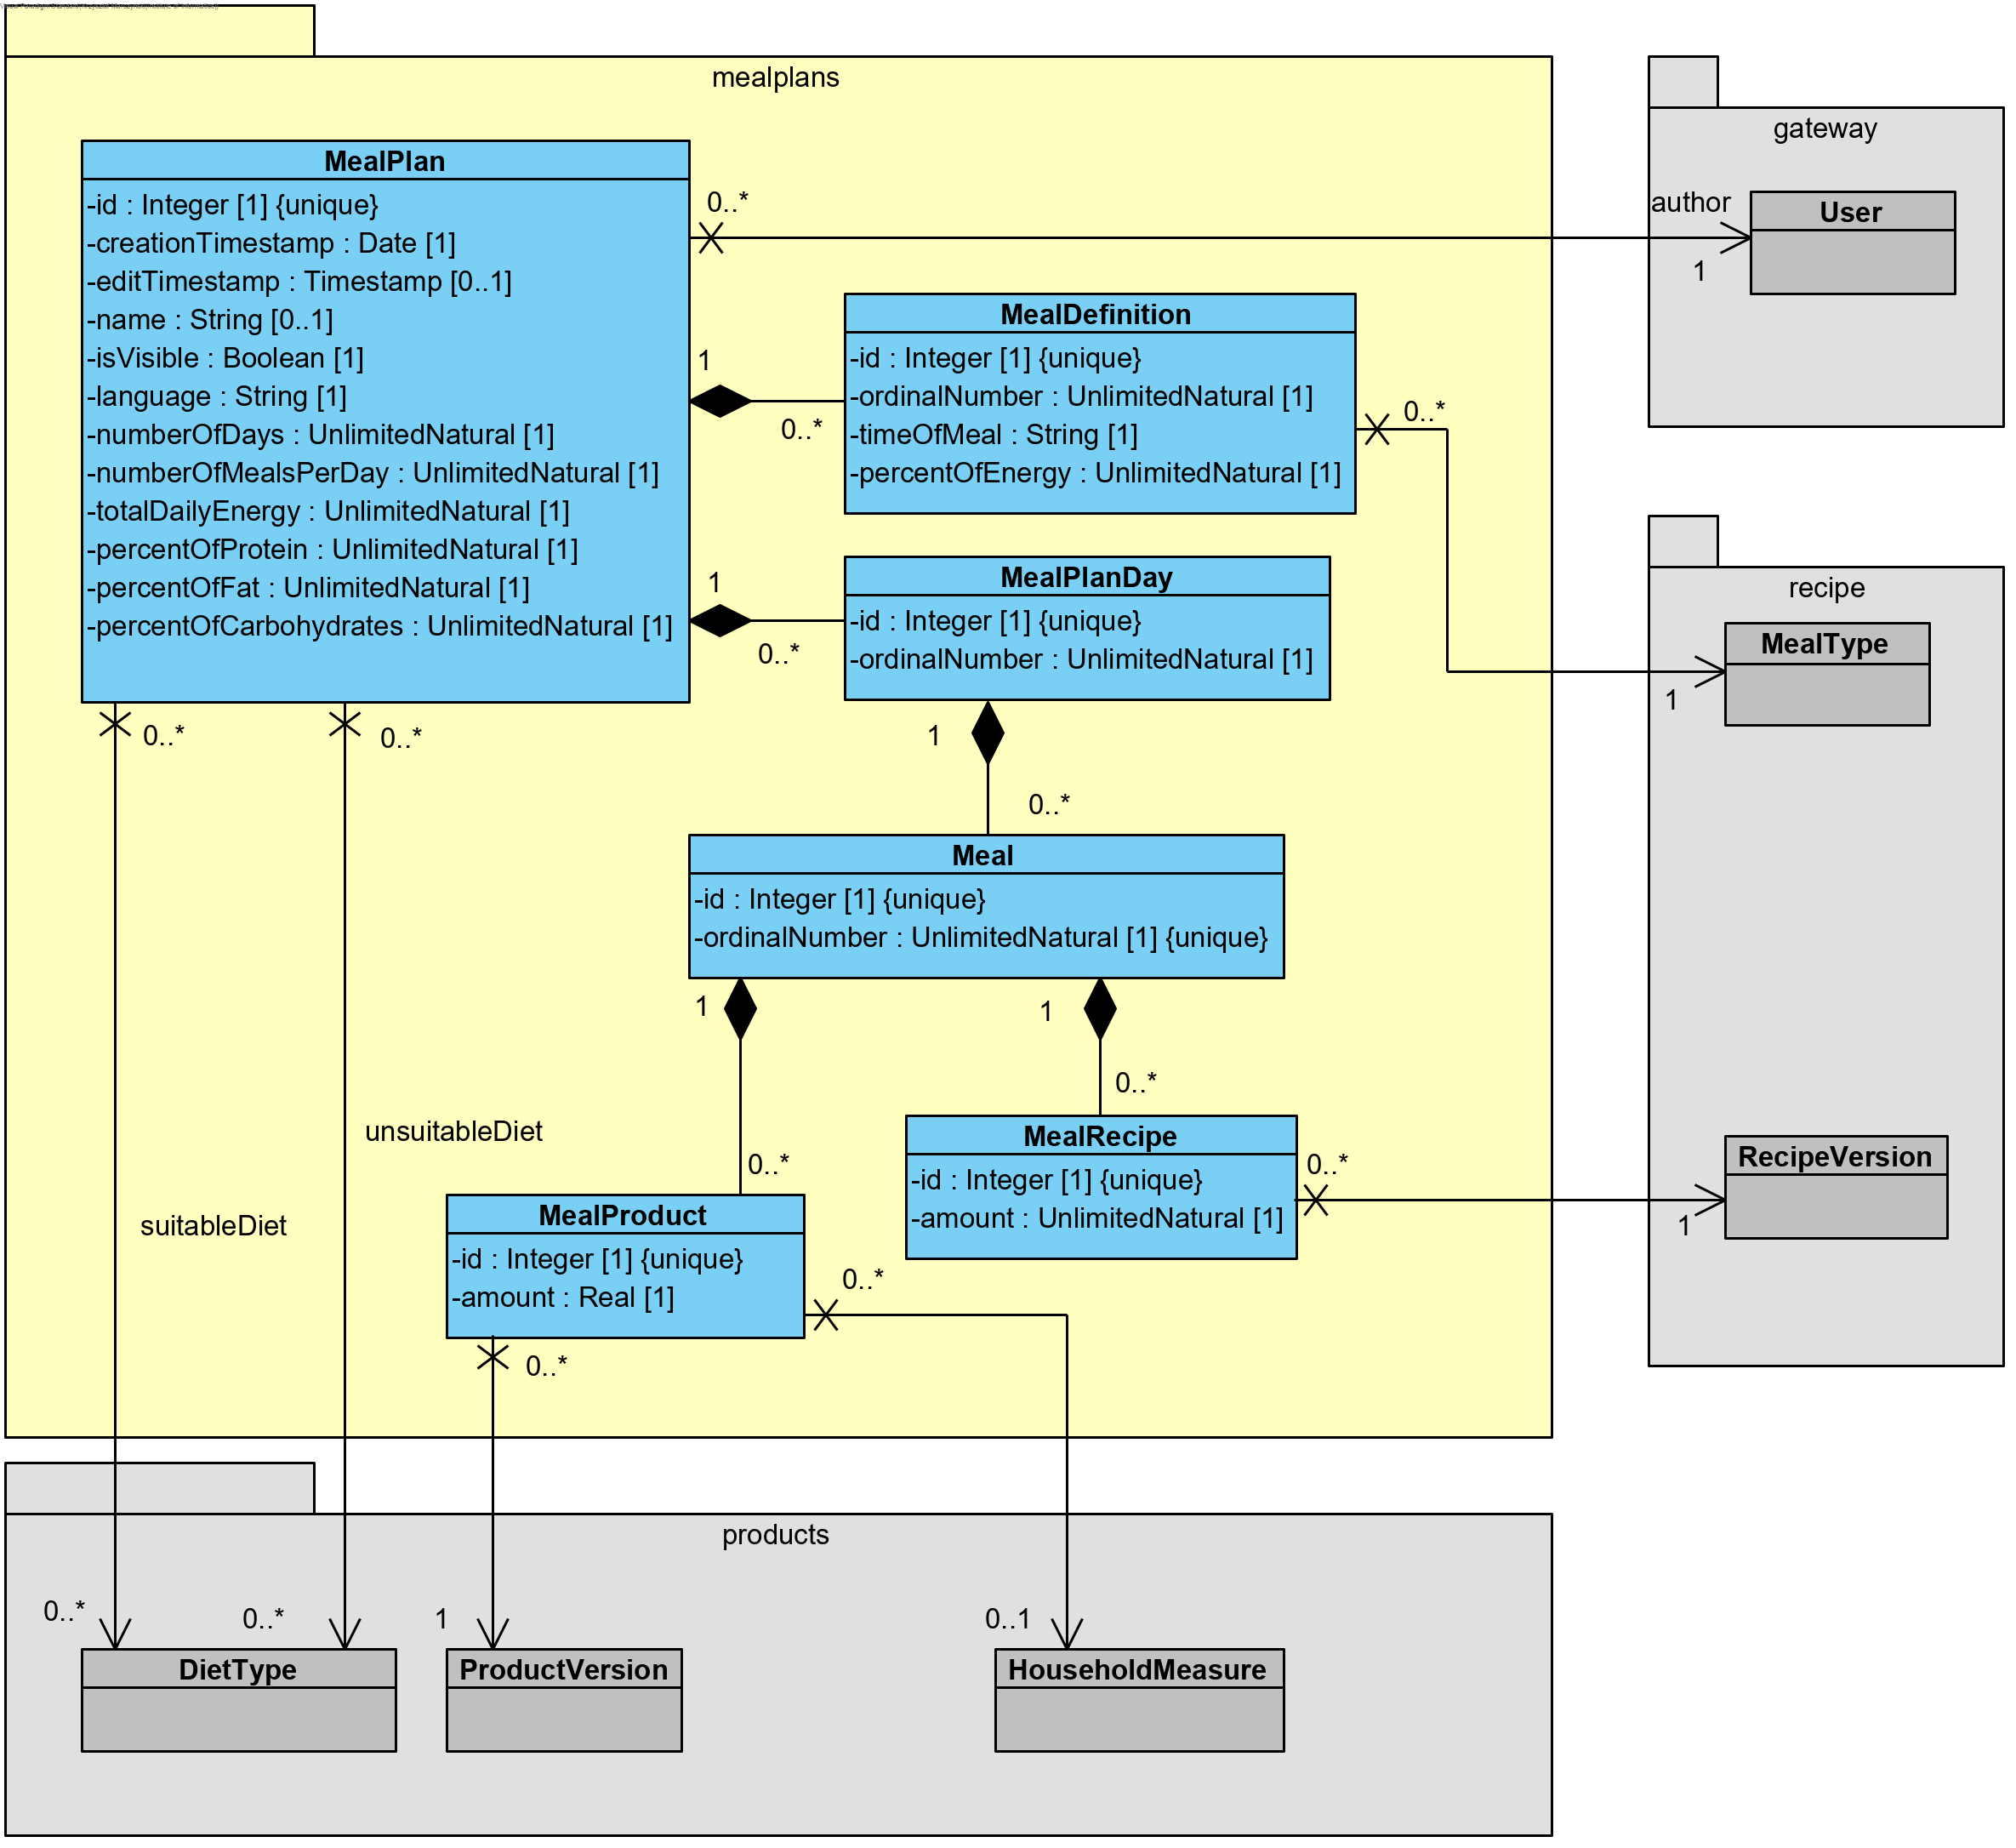
\includegraphics[scale=0.6]{../uml/class_diagrams/mealplans.png}
        \caption{Jadłospisy (opr.wł).}\label{rysunek:class-diagram-mealplans}
    \end{figure}
\end{minipage}

\begin{minipage}{\textwidth}
    \begin{figure}[H]
        \centering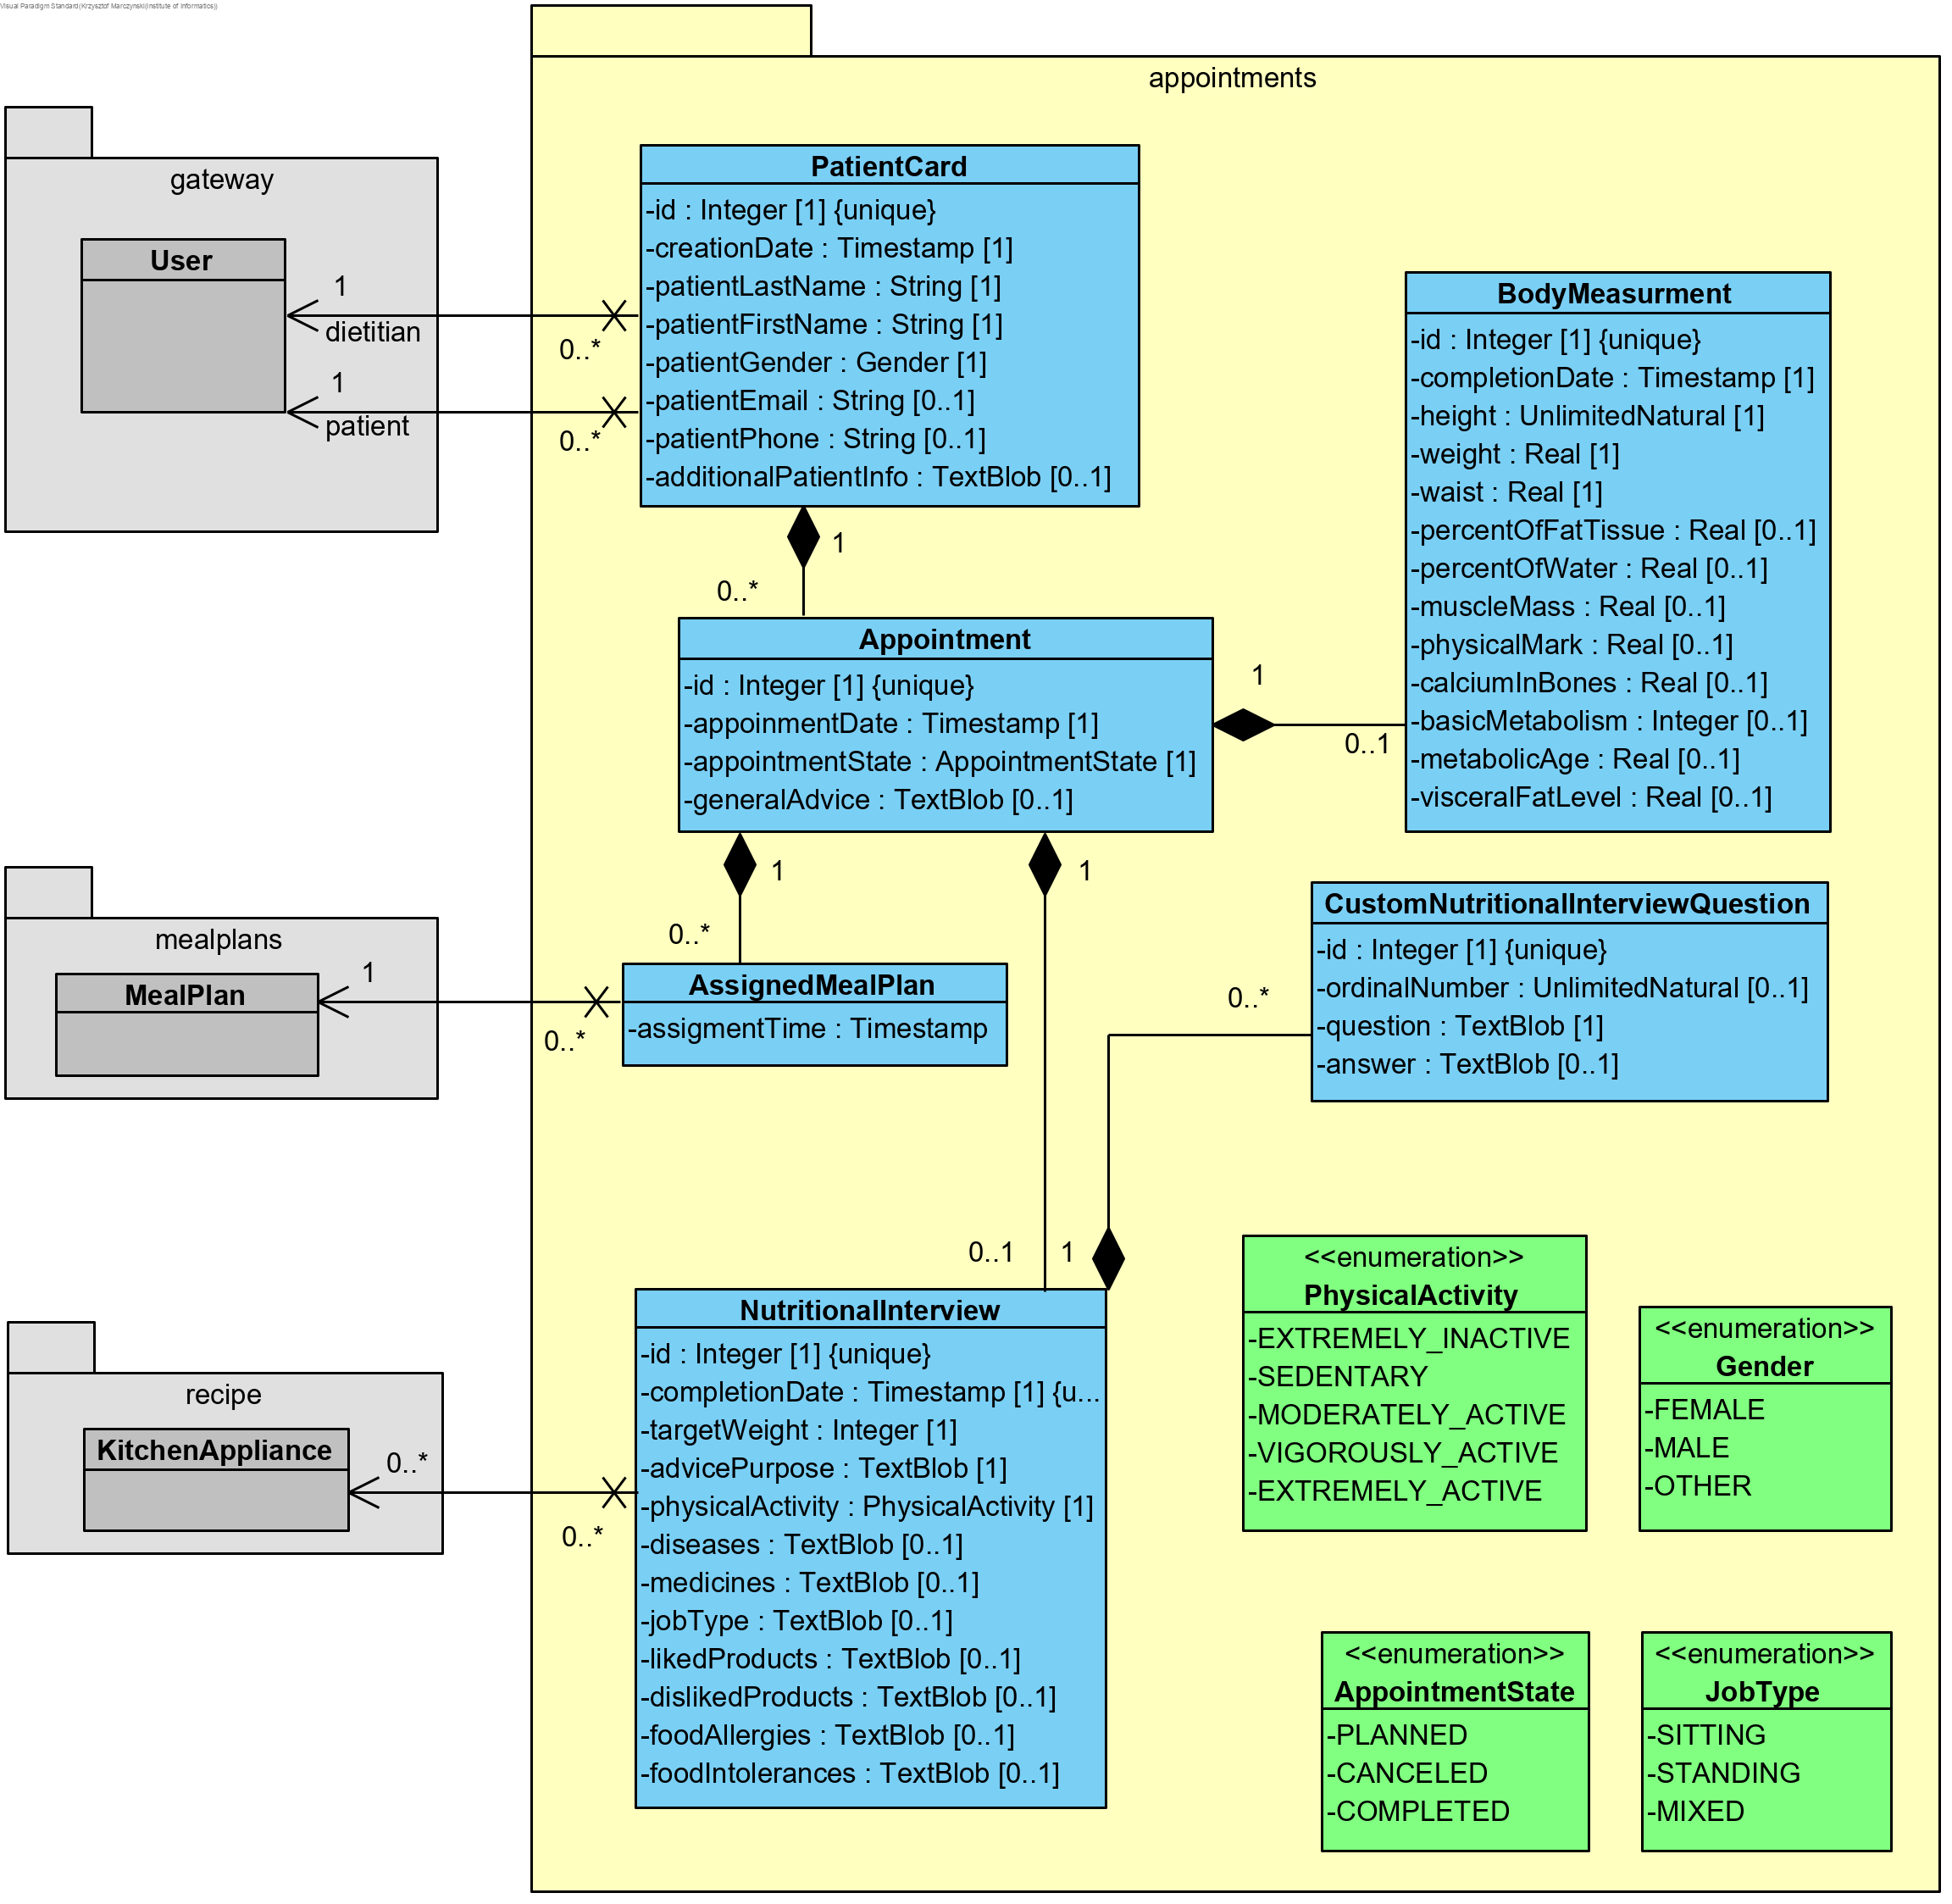
\includegraphics[scale=0.6]{../uml/class_diagrams/appointments.png}
        \caption{Wizyty (opr.wł).}\label{rysunek:class-diagram-appointments}
    \end{figure}
\end{minipage}

\section{Prototyp interfejsu}
\todo{mockupy}
\begin{minipage}{\textwidth}
    \begin{figure}[H]
        \centering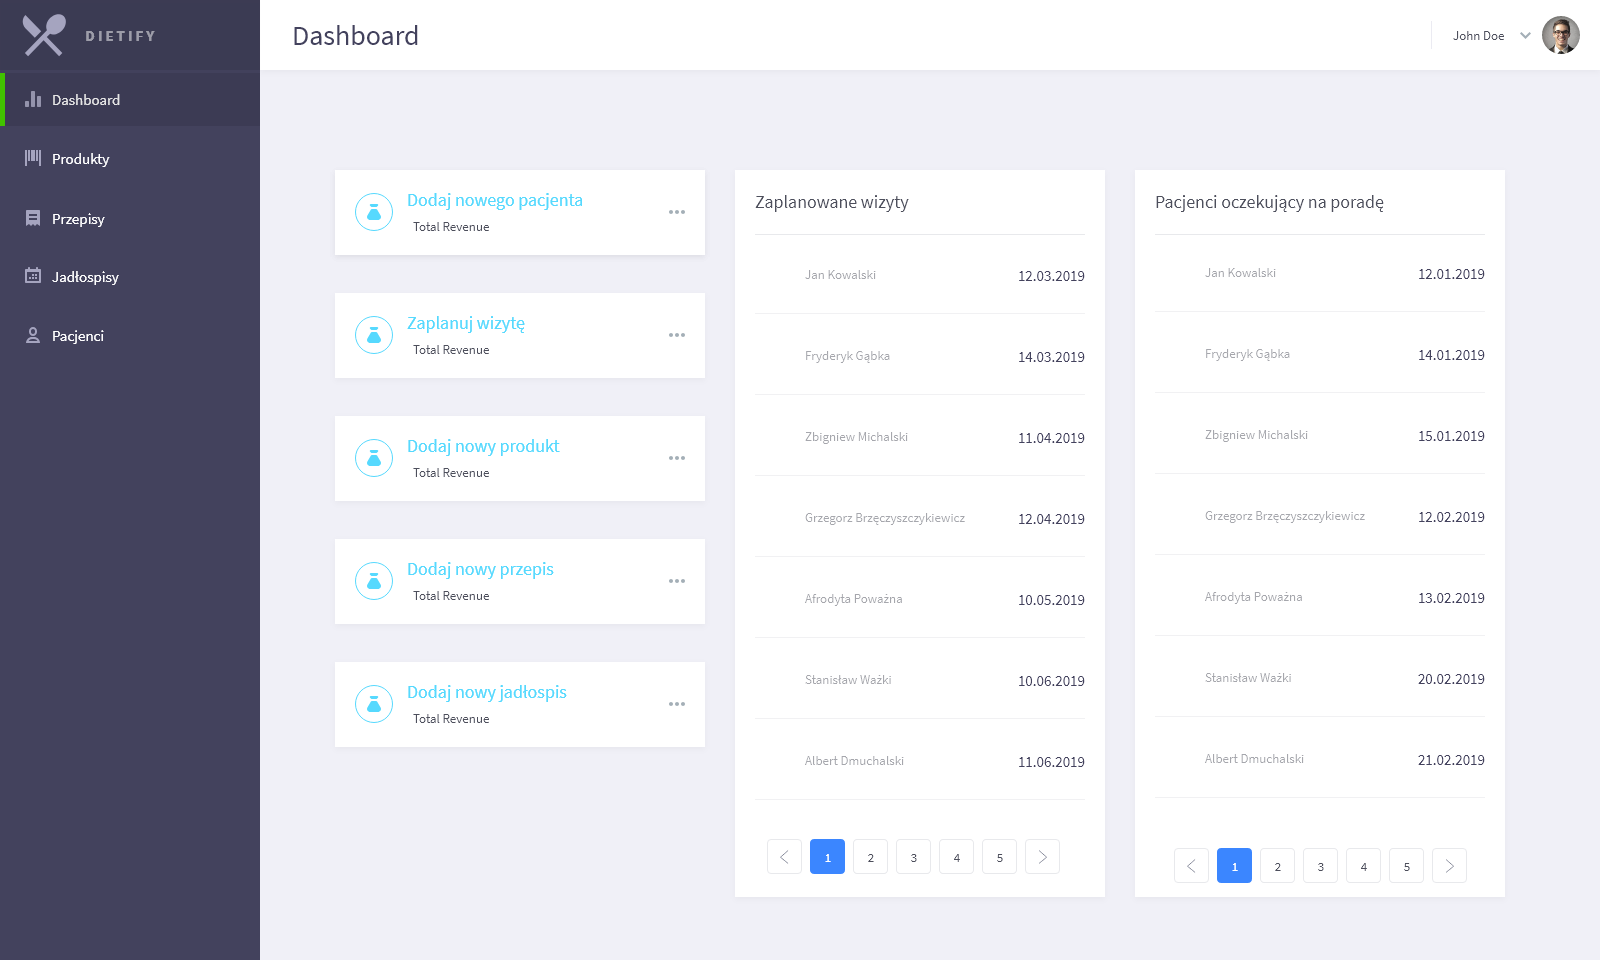
\includegraphics[width=0.9\textwidth]{img/mockups/mockup1.png}
        \caption{Mockup1 (opr.wł).}\label{rysunek:mockup1}
    \end{figure}
\end{minipage}

\begin{minipage}{\textwidth}
    \begin{figure}[H]
        \centering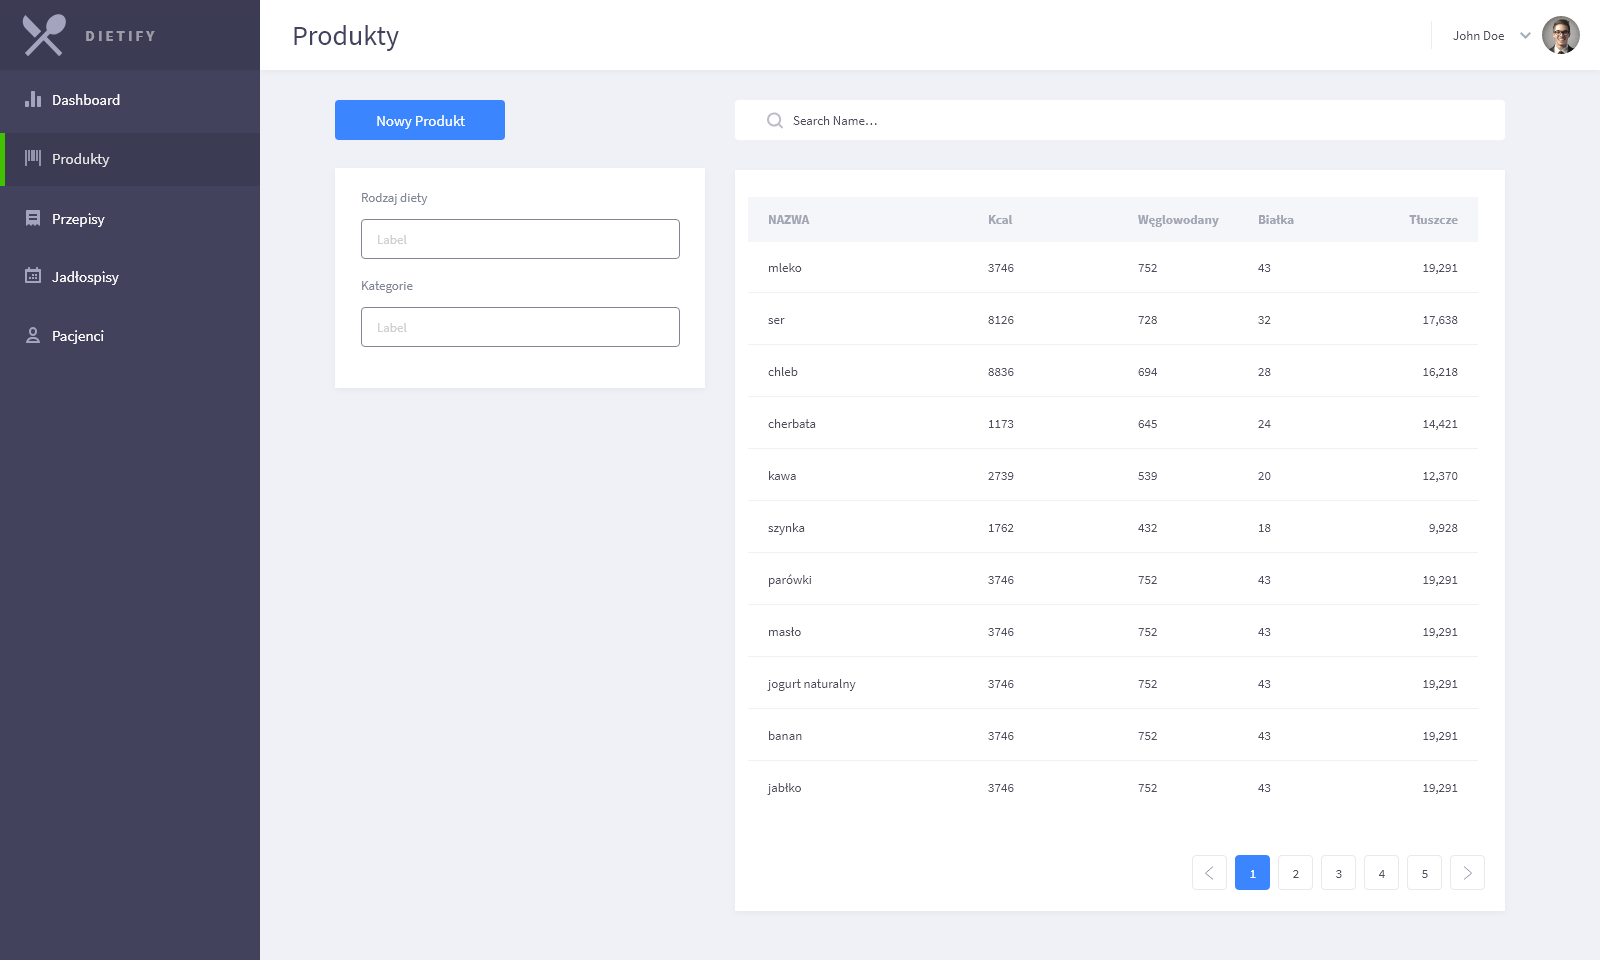
\includegraphics[width=0.9\textwidth]{img/mockups/mockup2.png}
        \caption{Mockup2 (opr.wł).}\label{rysunek:mockup2}
    \end{figure}
\end{minipage}

\begin{minipage}{\textwidth}
    \begin{figure}[H]
        \centering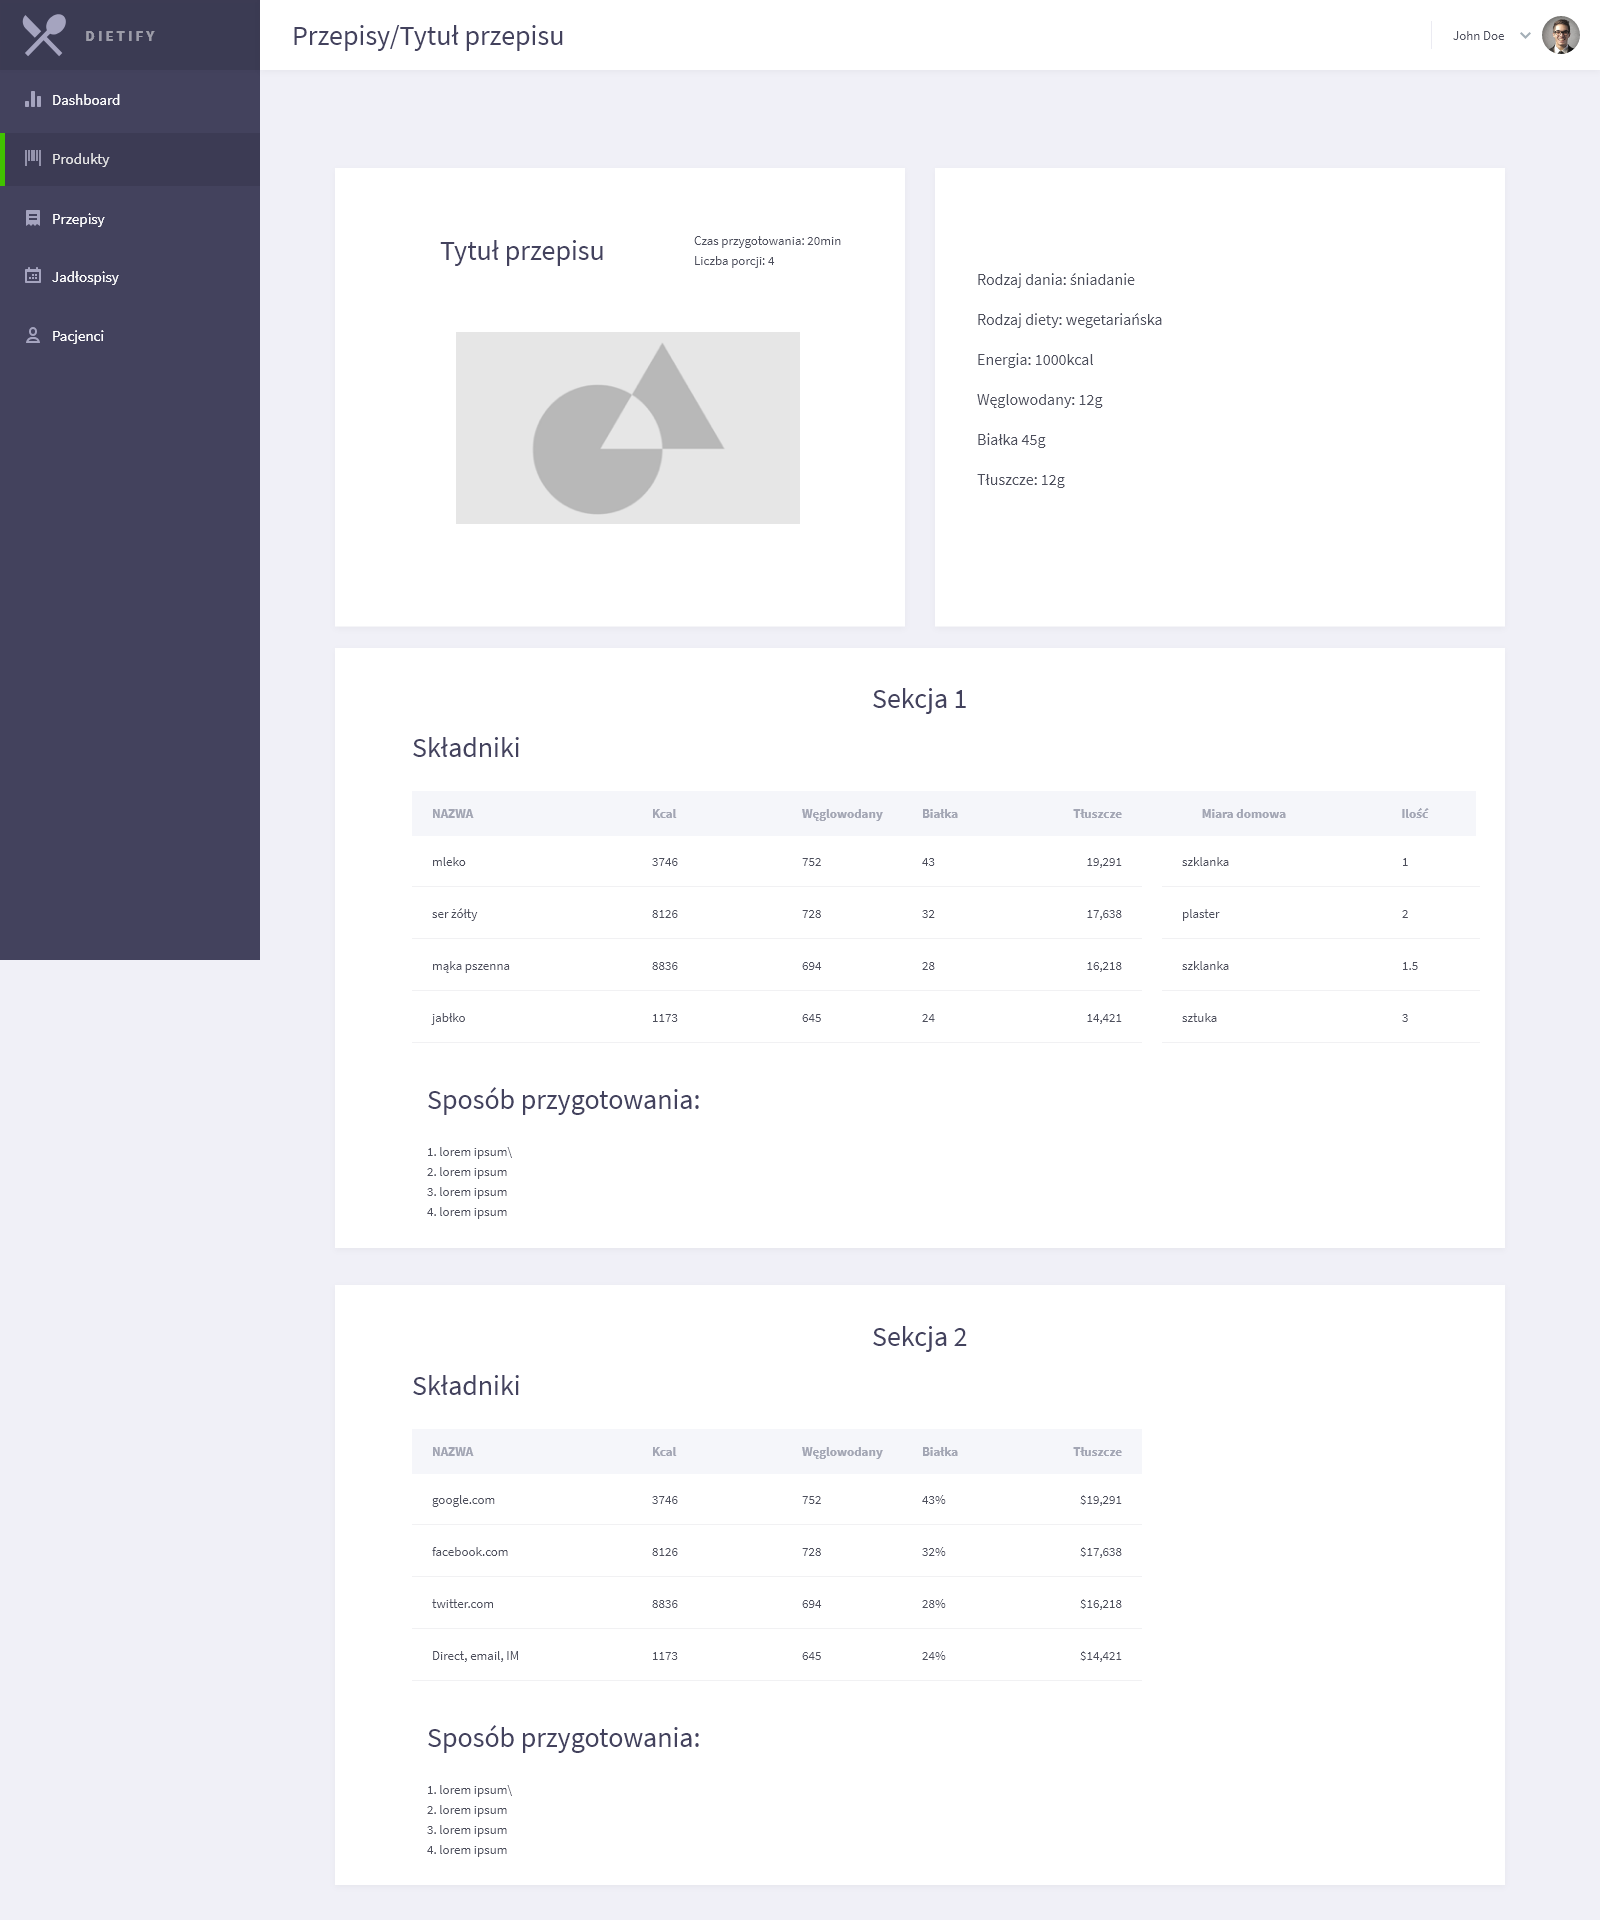
\includegraphics[width=0.9\textwidth]{img/mockups/mockup3.png}
        \caption{Mockup3 (opr.wł).}\label{rysunek:mockup3}
    \end{figure}
\end{minipage}

\begin{minipage}{\textwidth}
    \begin{figure}[H]
        \centering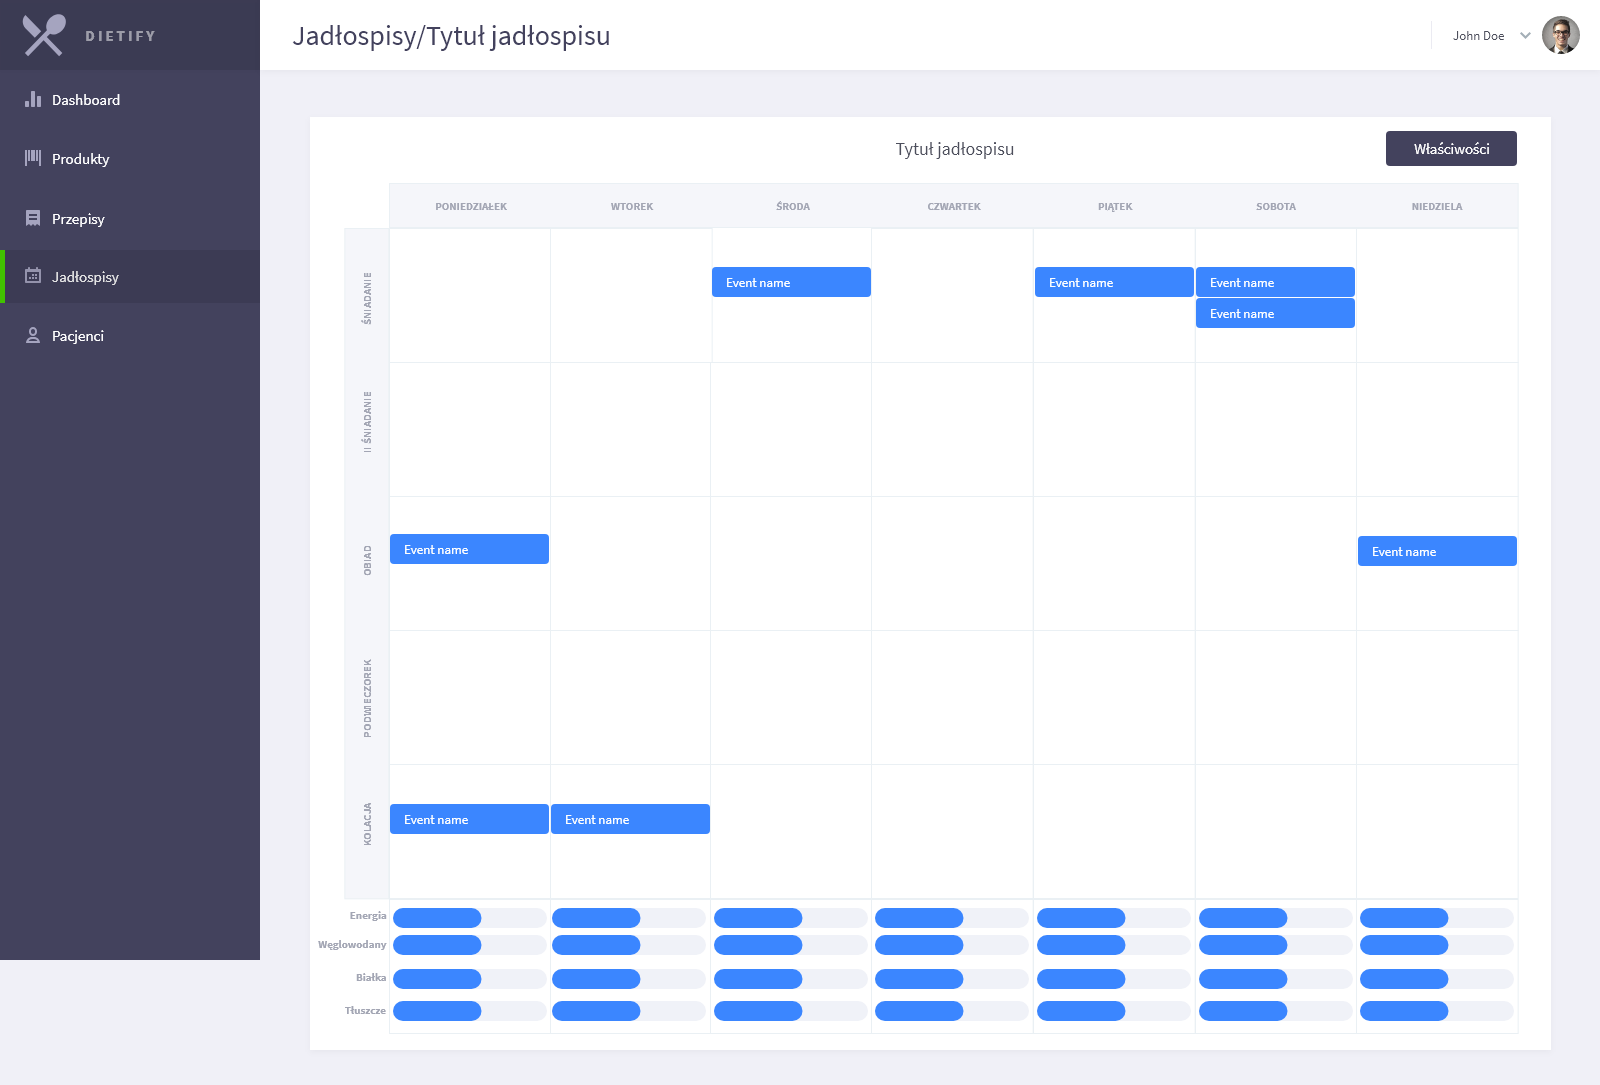
\includegraphics[width=0.9\textwidth]{img/mockups/mockup4.png}
        \caption{Mockup4 (opr.wł).}\label{rysunek:mockup4}
    \end{figure}
\end{minipage}

\begin{minipage}{\textwidth}
    \begin{figure}[H]
        \centering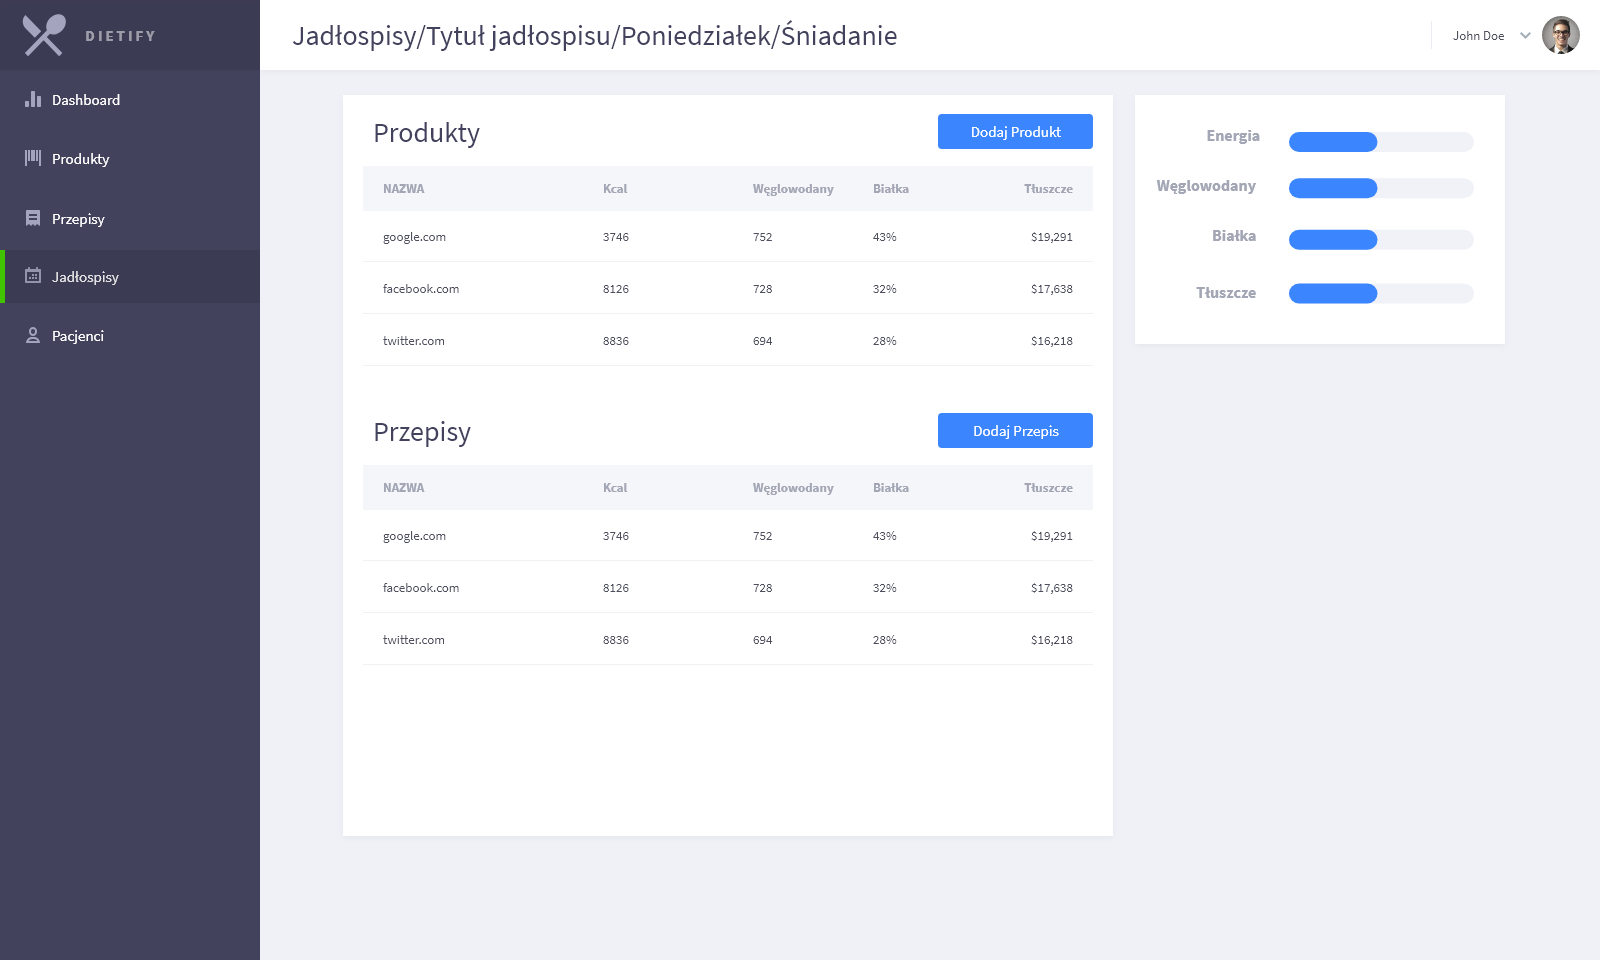
\includegraphics[width=0.9\textwidth]{img/mockups/mockup5.png}
        \caption{Mockup5 (opr.wł).}\label{rysunek:mockup5}
    \end{figure}
\end{minipage}

\begin{minipage}{\textwidth}
    \begin{figure}[H]
        \centering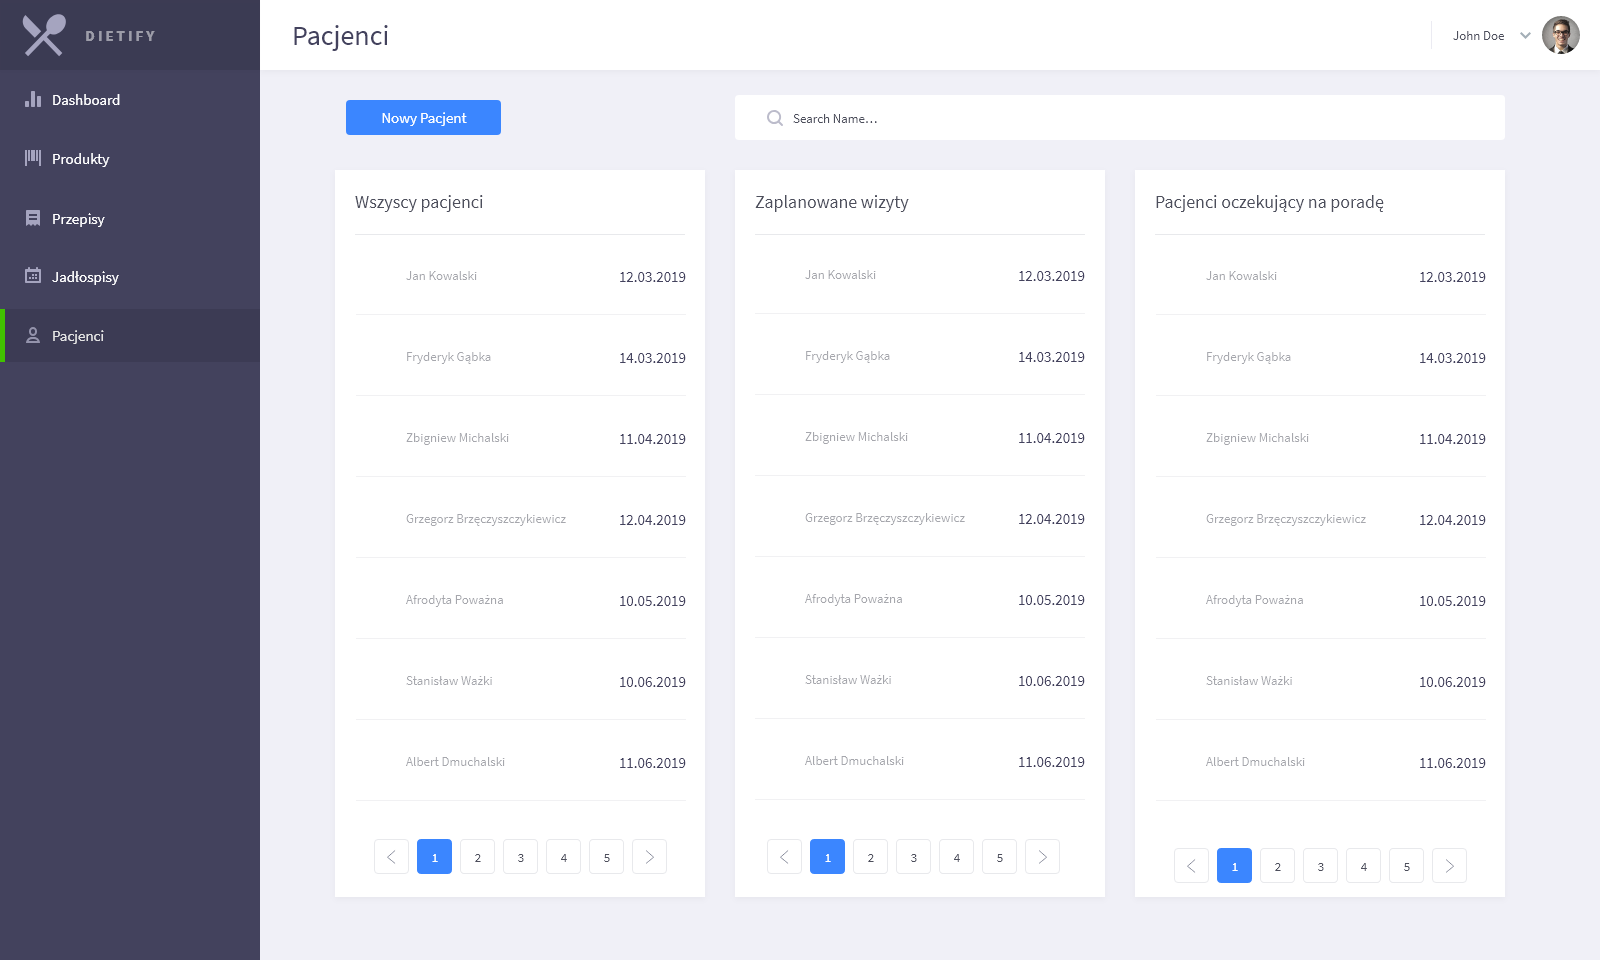
\includegraphics[width=0.9\textwidth]{img/mockups/mockup6.png}
        \caption{Mockup6 (opr.wł).}\label{rysunek:mockup6}
    \end{figure}
\end{minipage}

\begin{minipage}{\textwidth}
    \begin{figure}[H]
        \centering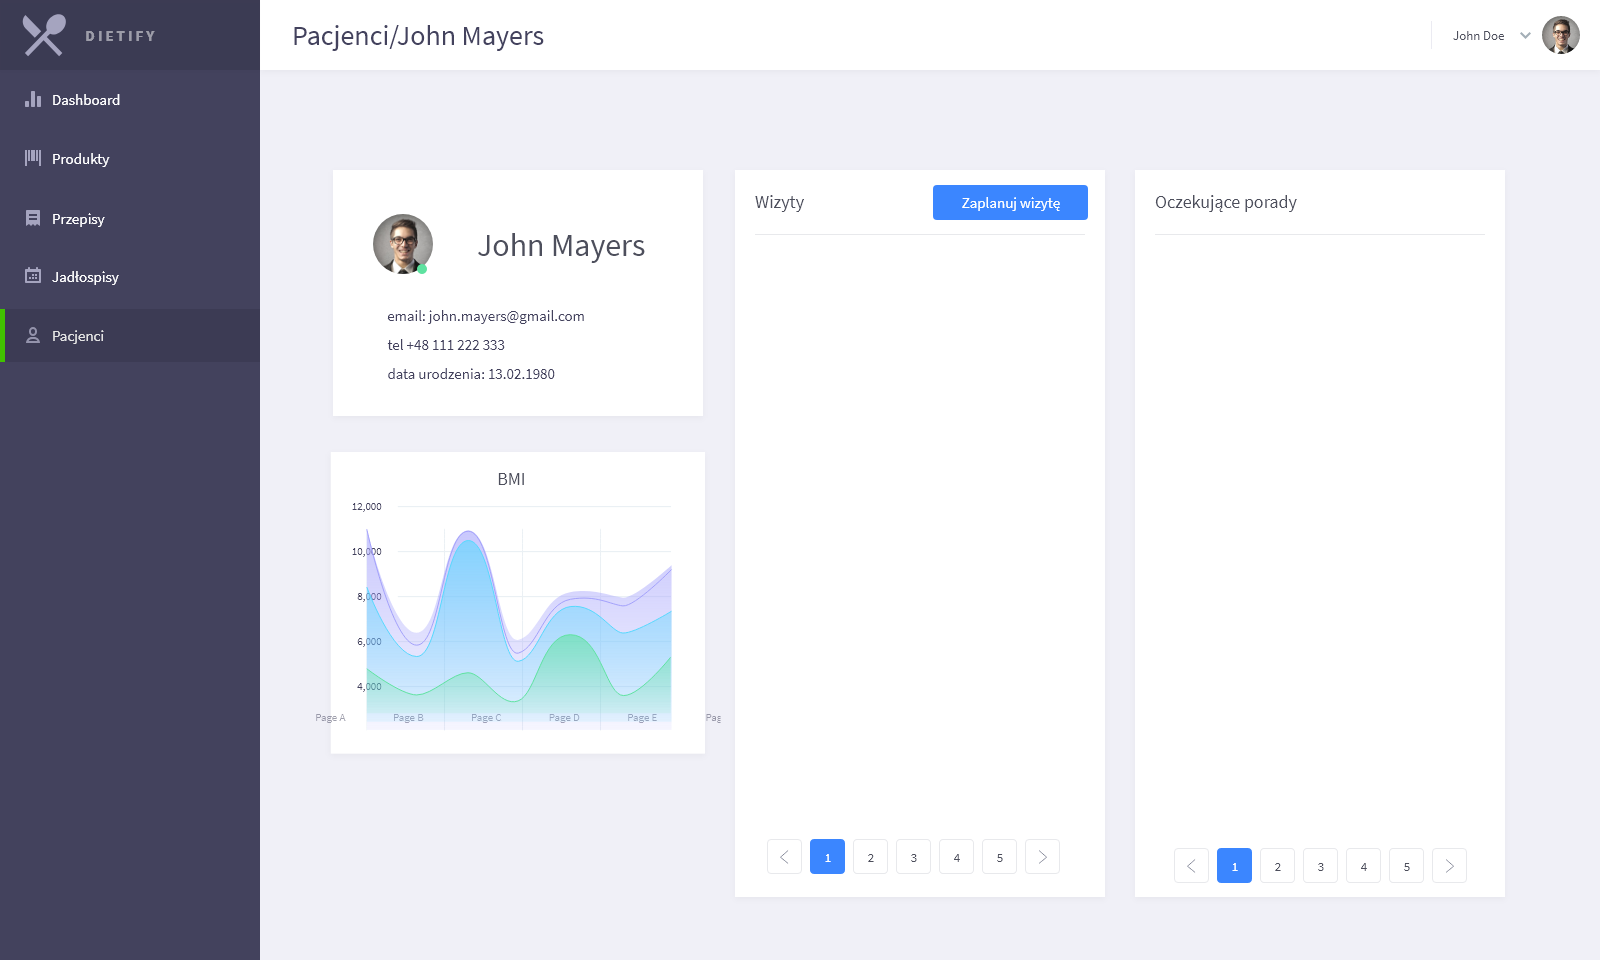
\includegraphics[width=0.9\textwidth]{img/mockups/mockup7.png}
        \caption{Mockup7 (opr.wł).}\label{rysunek:mockup7}
    \end{figure}
\end{minipage}

\begin{minipage}{\textwidth}
    \begin{figure}[H]
        \centering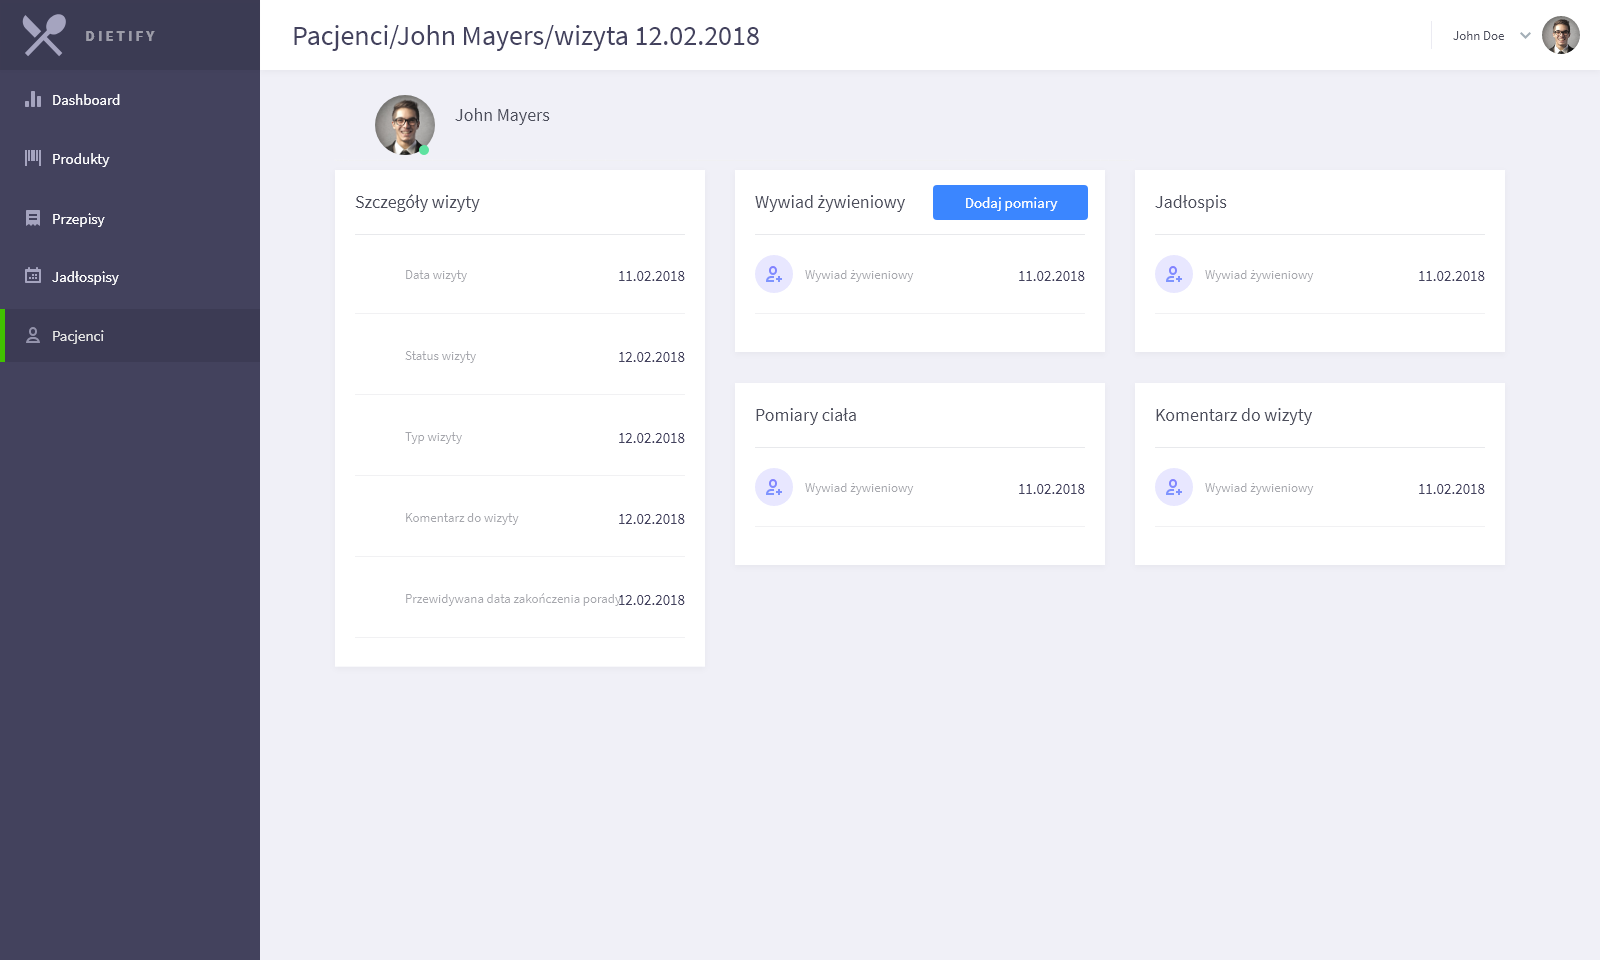
\includegraphics[width=0.9\textwidth]{img/mockups/mockup8.png}
        \caption{Mockup8 (opr.wł).}\label{rysunek:mockup8}
    \end{figure}
\end{minipage}

\begin{minipage}{\textwidth}
    \begin{figure}[H]
        \centering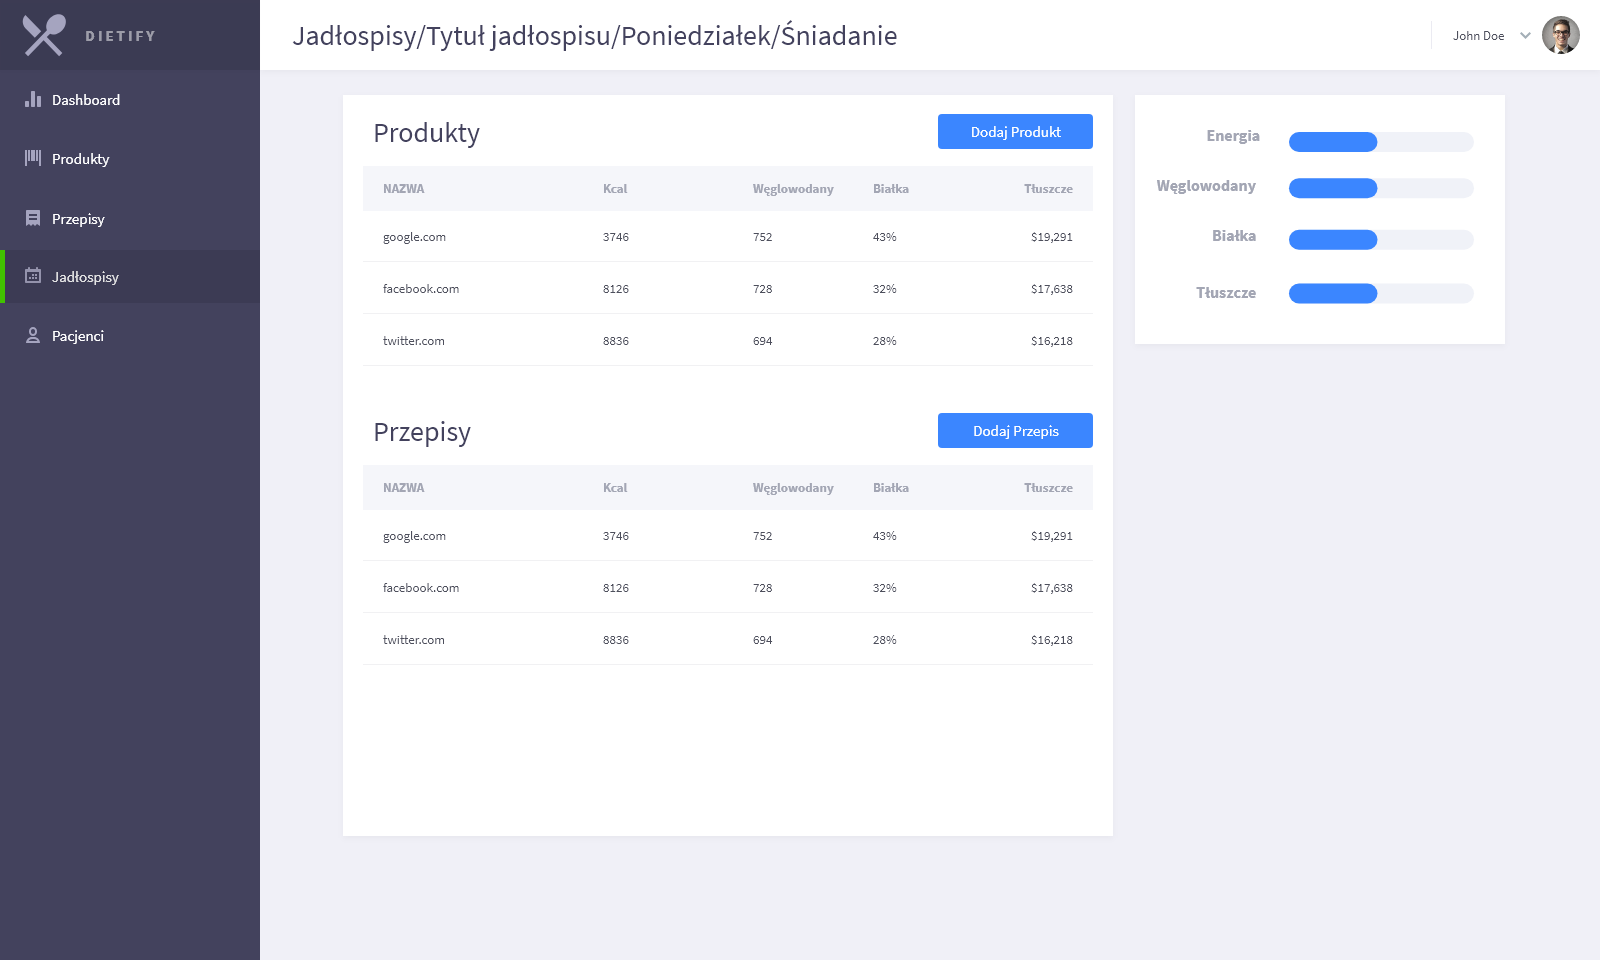
\includegraphics[width=0.9\textwidth]{img/mockups/mockup9.png}
        \caption{Mockup9 (opr.wł).}\label{rysunek:mockup9}
    \end{figure}
\end{minipage}

\begin{minipage}{\textwidth}
    \begin{figure}[H]
        \centering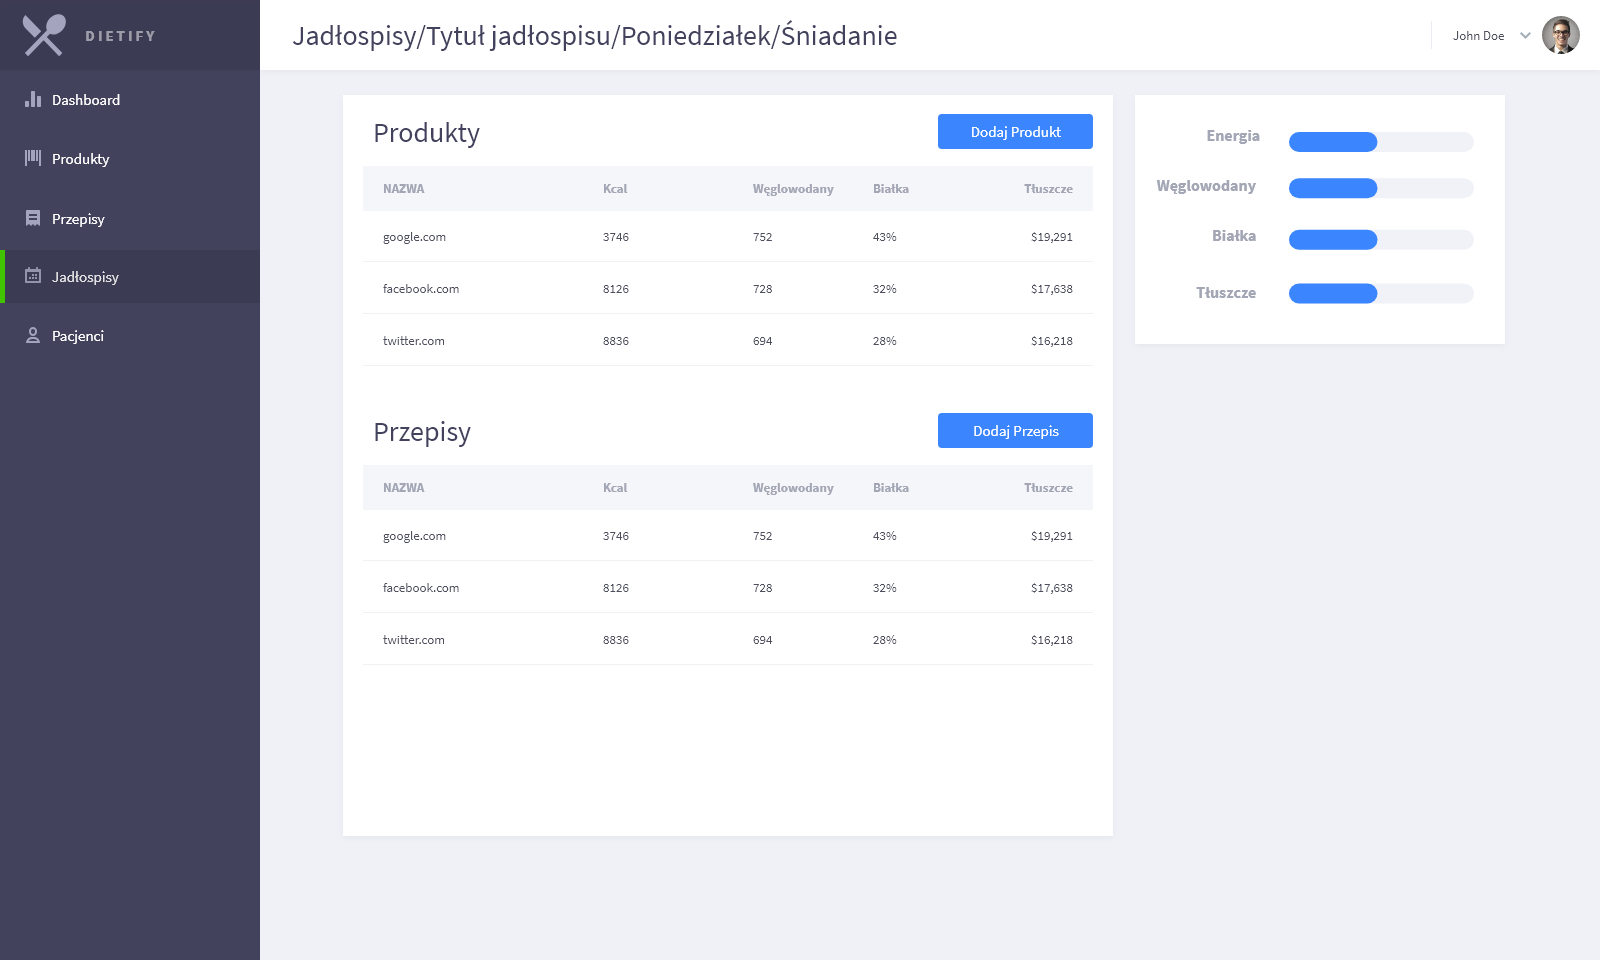
\includegraphics[width=0.9\textwidth]{img/mockups/mockup10.png}
        \caption{Mockup10 (opr.wł).}\label{rysunek:mockup10}
    \end{figure}
\end{minipage}

\begin{minipage}{\textwidth}
    \begin{figure}[H]
        \centering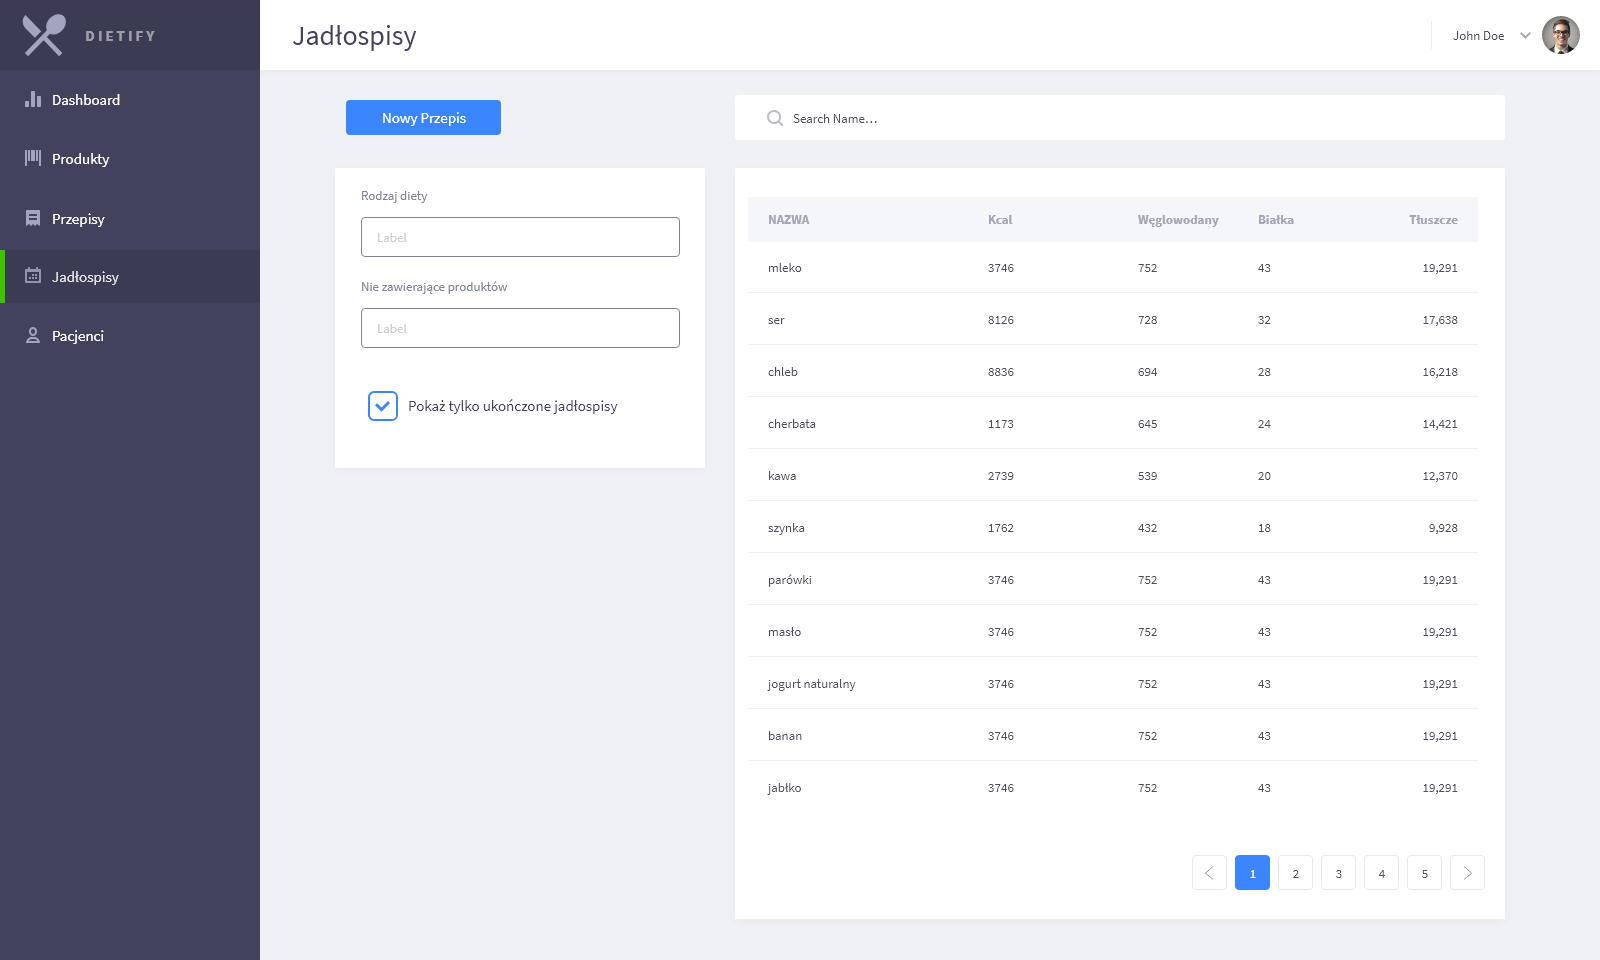
\includegraphics[width=0.9\textwidth]{img/mockups/mockup11.png}
        \caption{Mockup11 (opr.wł).}\label{rysunek:mockup11}
    \end{figure}
\end{minipage}

\begin{minipage}{\textwidth}
    \begin{figure}[H]
        \centering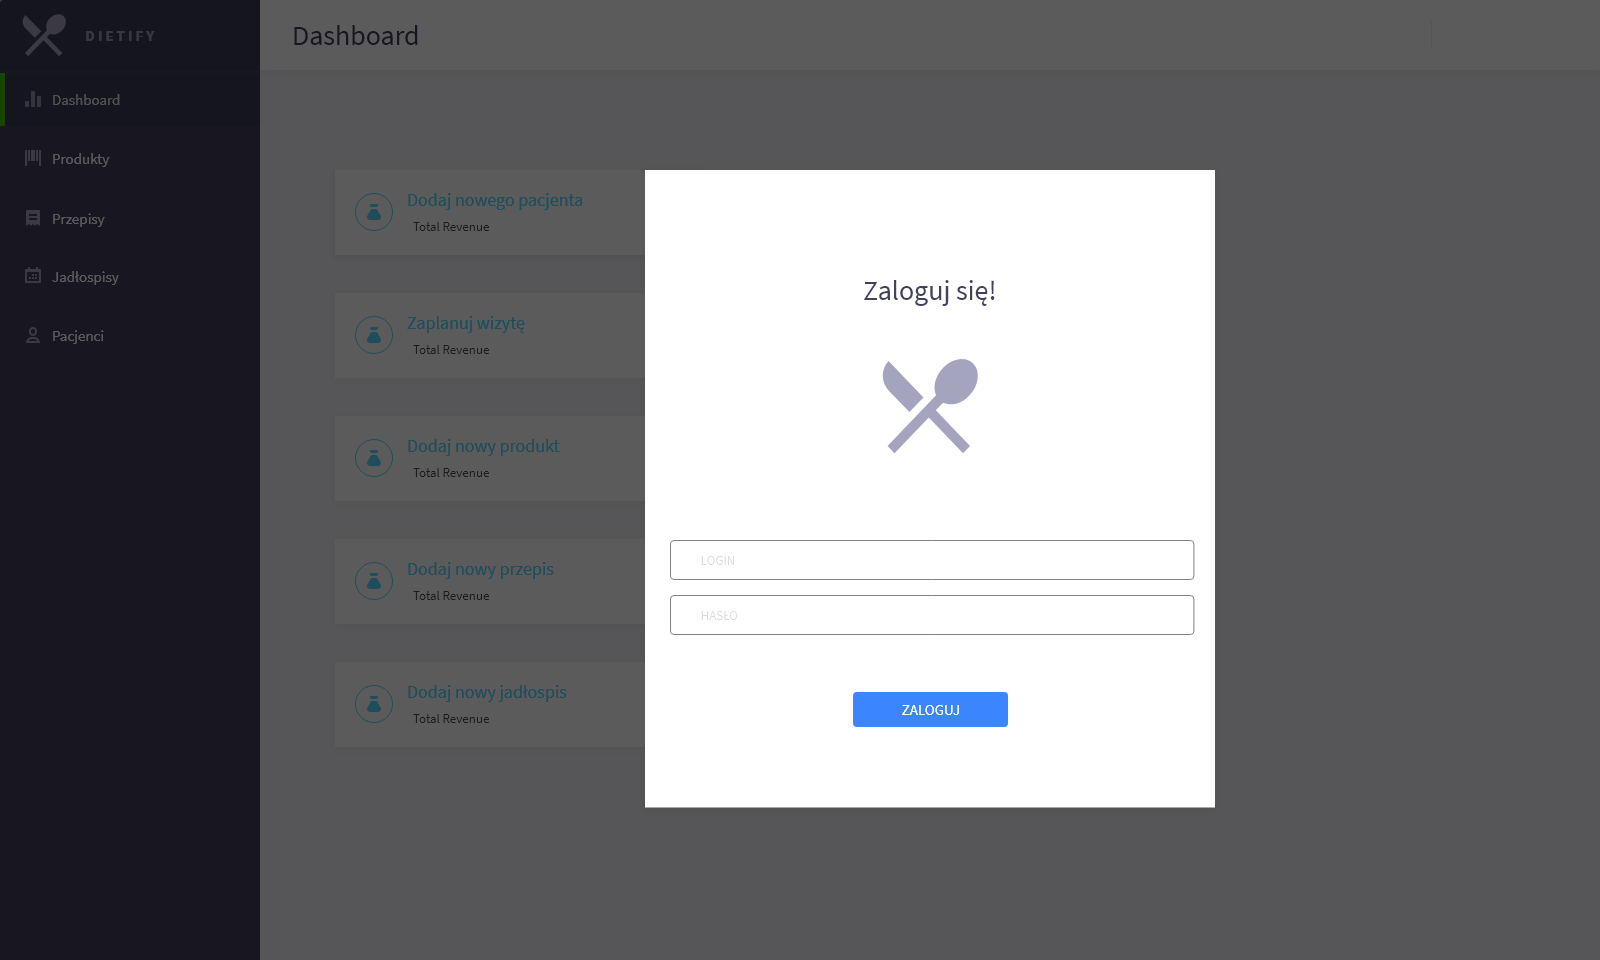
\includegraphics[width=0.9\textwidth]{img/mockups/mockup12.png}
        \caption{Mockup12 (opr.wł).}\label{rysunek:mockup12}
    \end{figure}
\end{minipage}

\begin{minipage}{\textwidth}
    \begin{figure}[H]
        \centering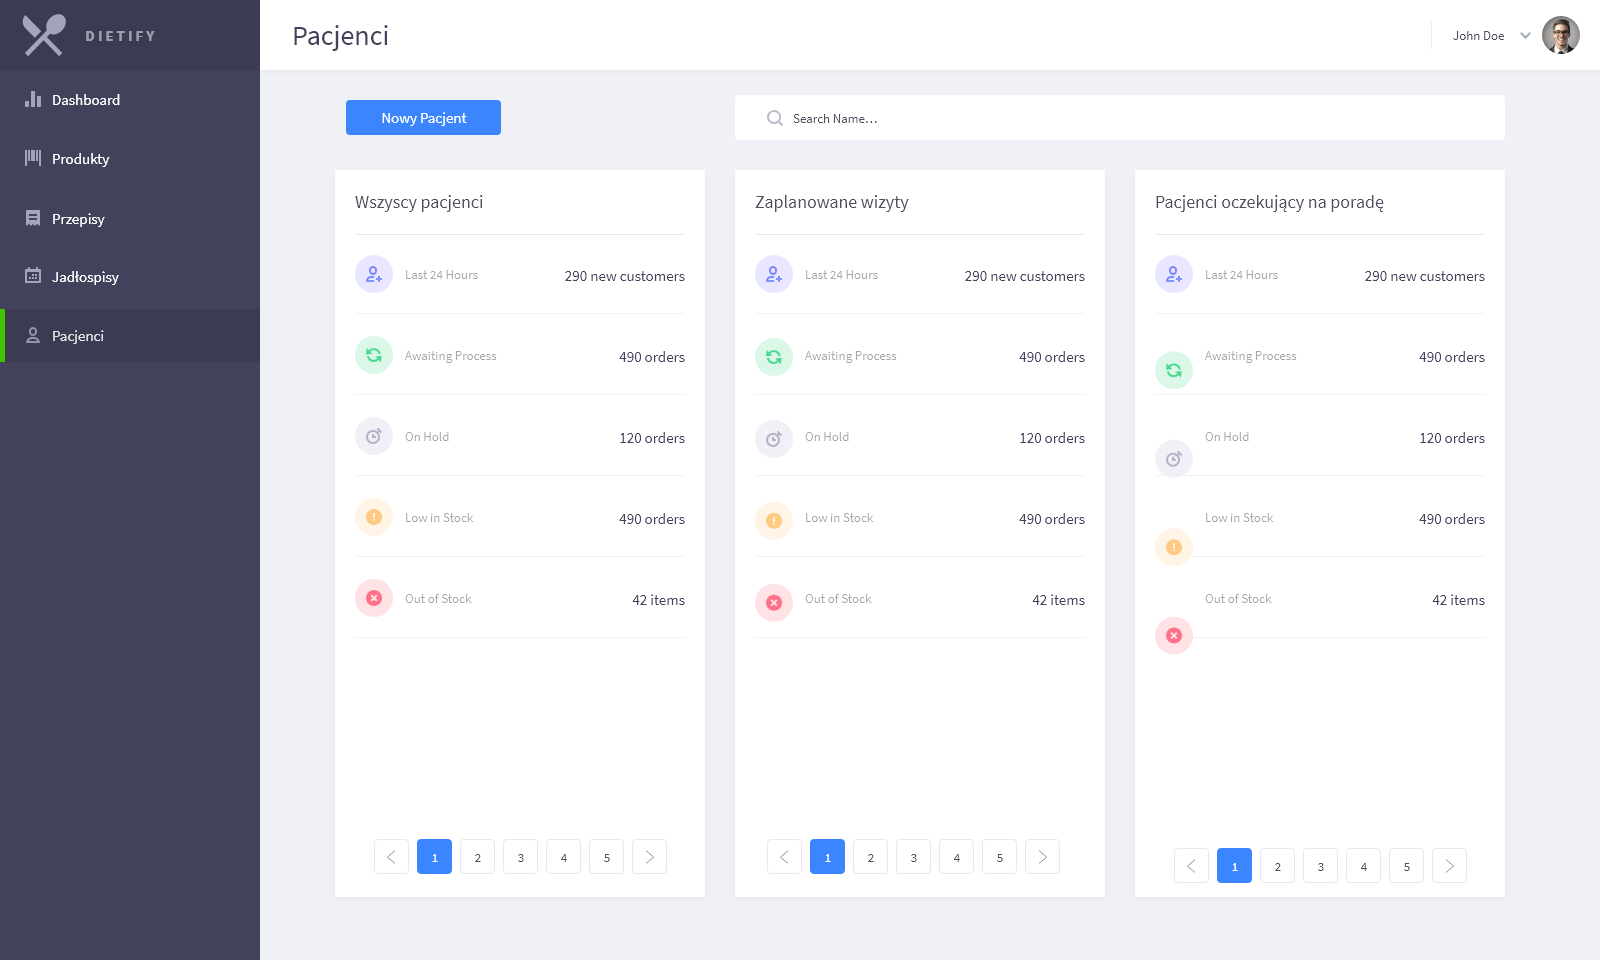
\includegraphics[width=0.9\textwidth]{img/mockups/mockup13.png}
        \caption{Mockup13 (opr.wł).}\label{rysunek:mockup13}
    \end{figure}
\end{minipage}

\begin{minipage}{\textwidth}
    \begin{figure}[H]
        \centering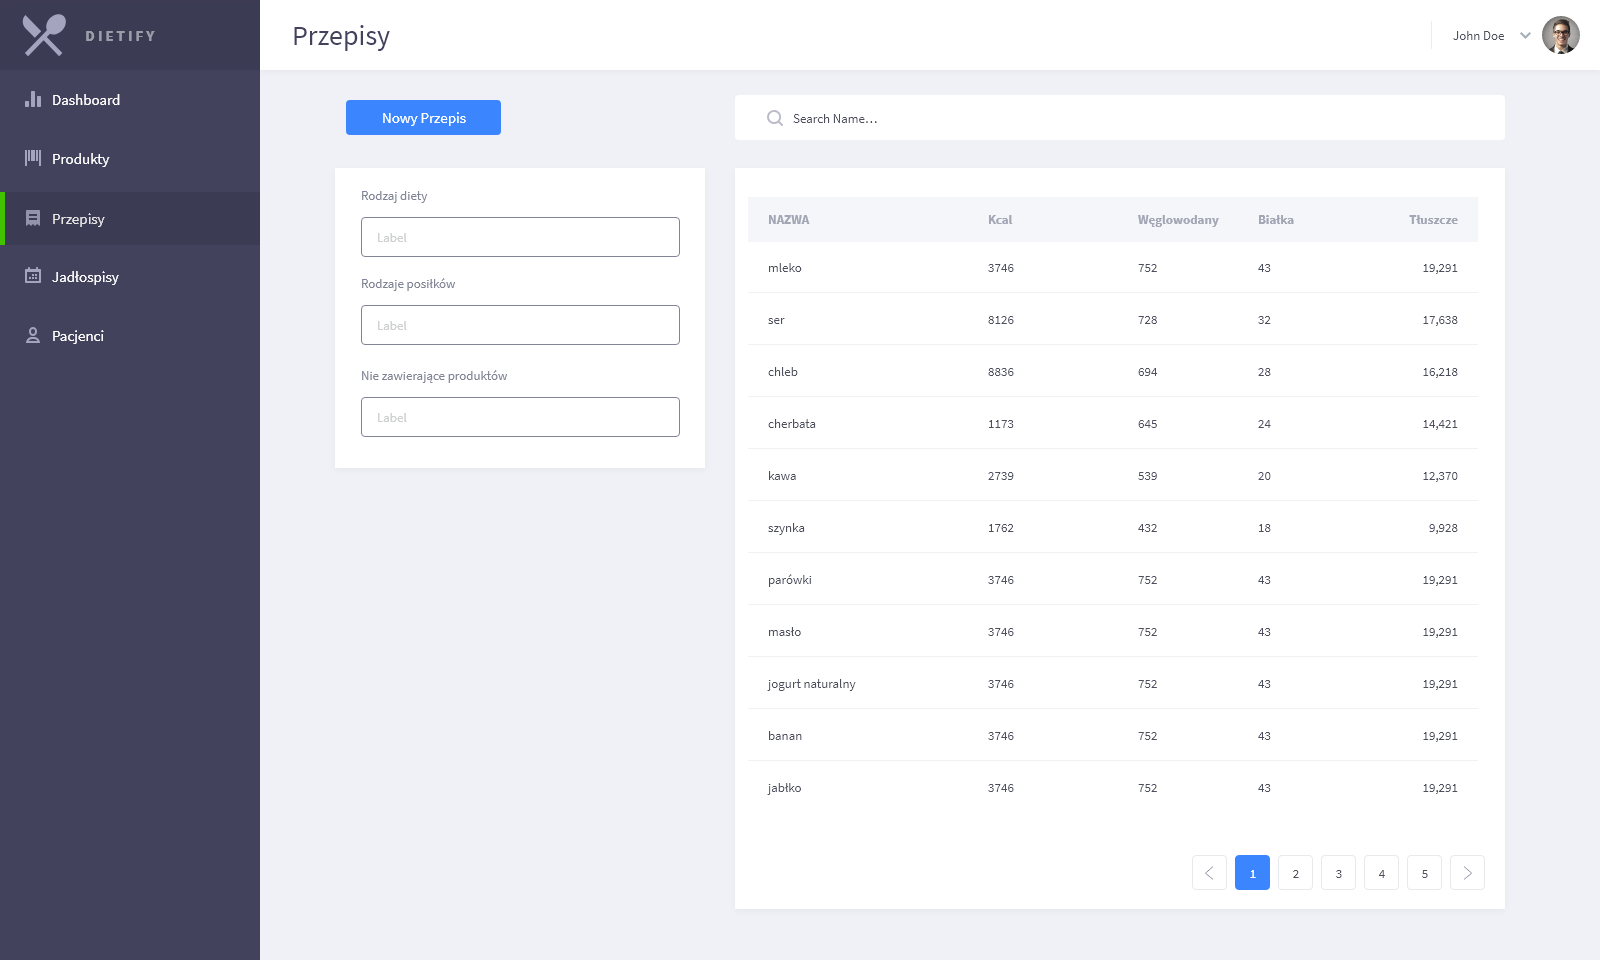
\includegraphics[width=0.9\textwidth]{img/mockups/mockup14.png}
        \caption{Mockup14 (opr.wł).}\label{rysunek:mockup14}
    \end{figure}
\end{minipage}

\begin{minipage}{\textwidth}
    \begin{figure}[H]
        \centering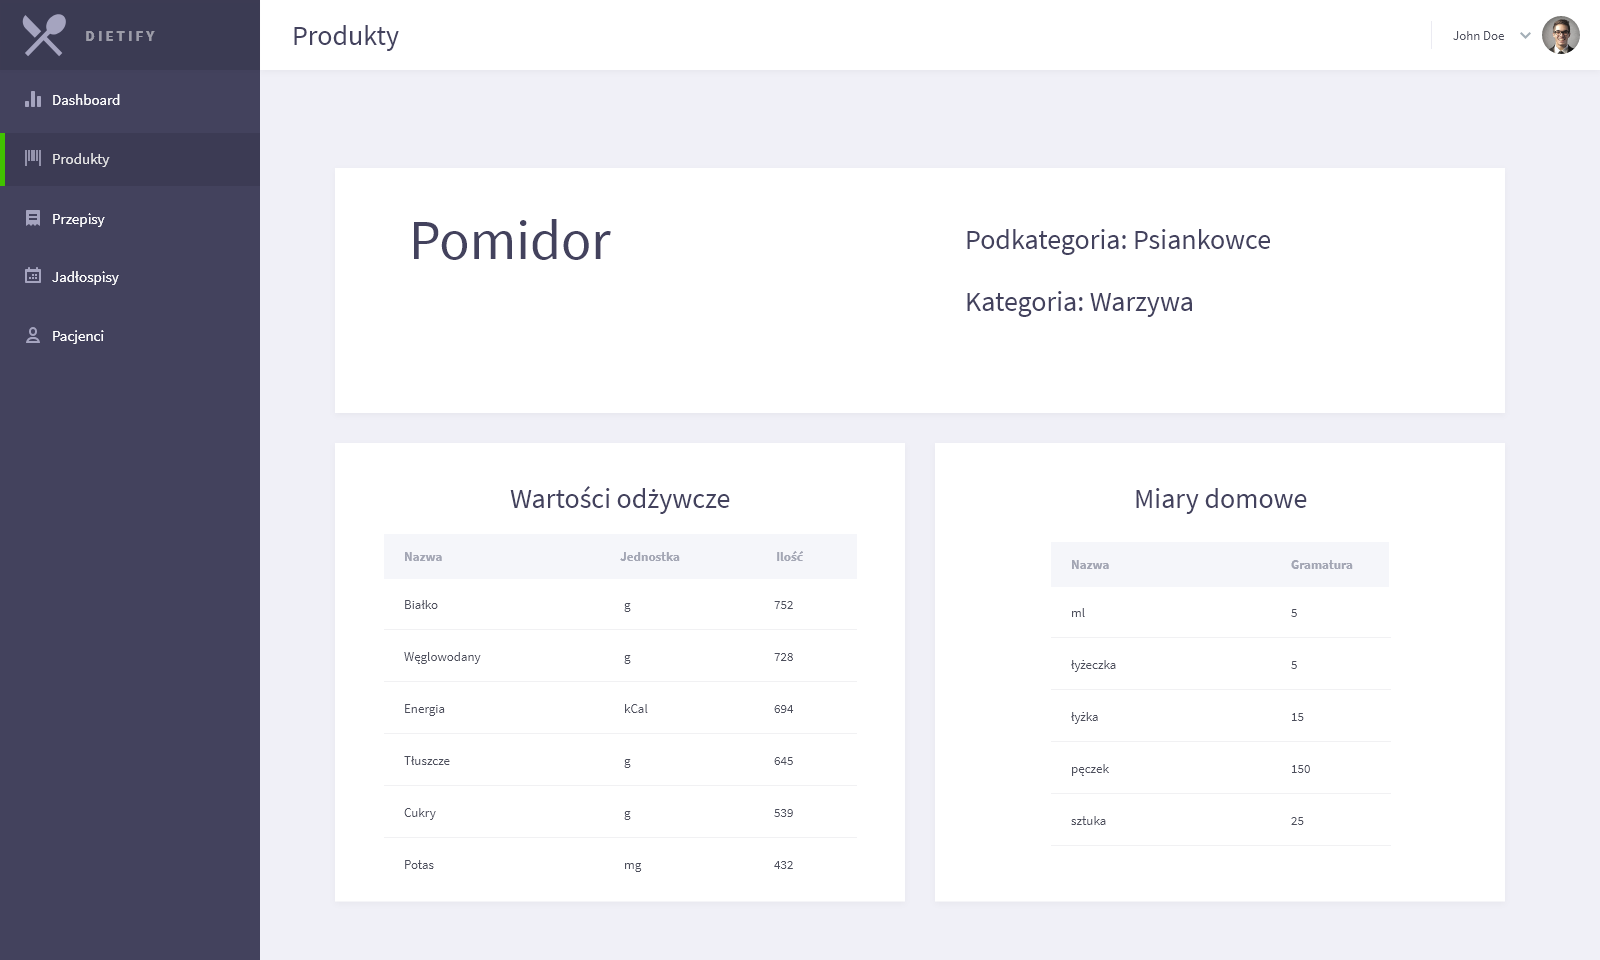
\includegraphics[width=0.9\textwidth]{img/mockups/mockup15.png}
        \caption{Mockup15 (opr.wł).}\label{rysunek:mockup15}
    \end{figure}
\end{minipage}

\begin{minipage}{\textwidth}
    \begin{figure}[H]
        \centering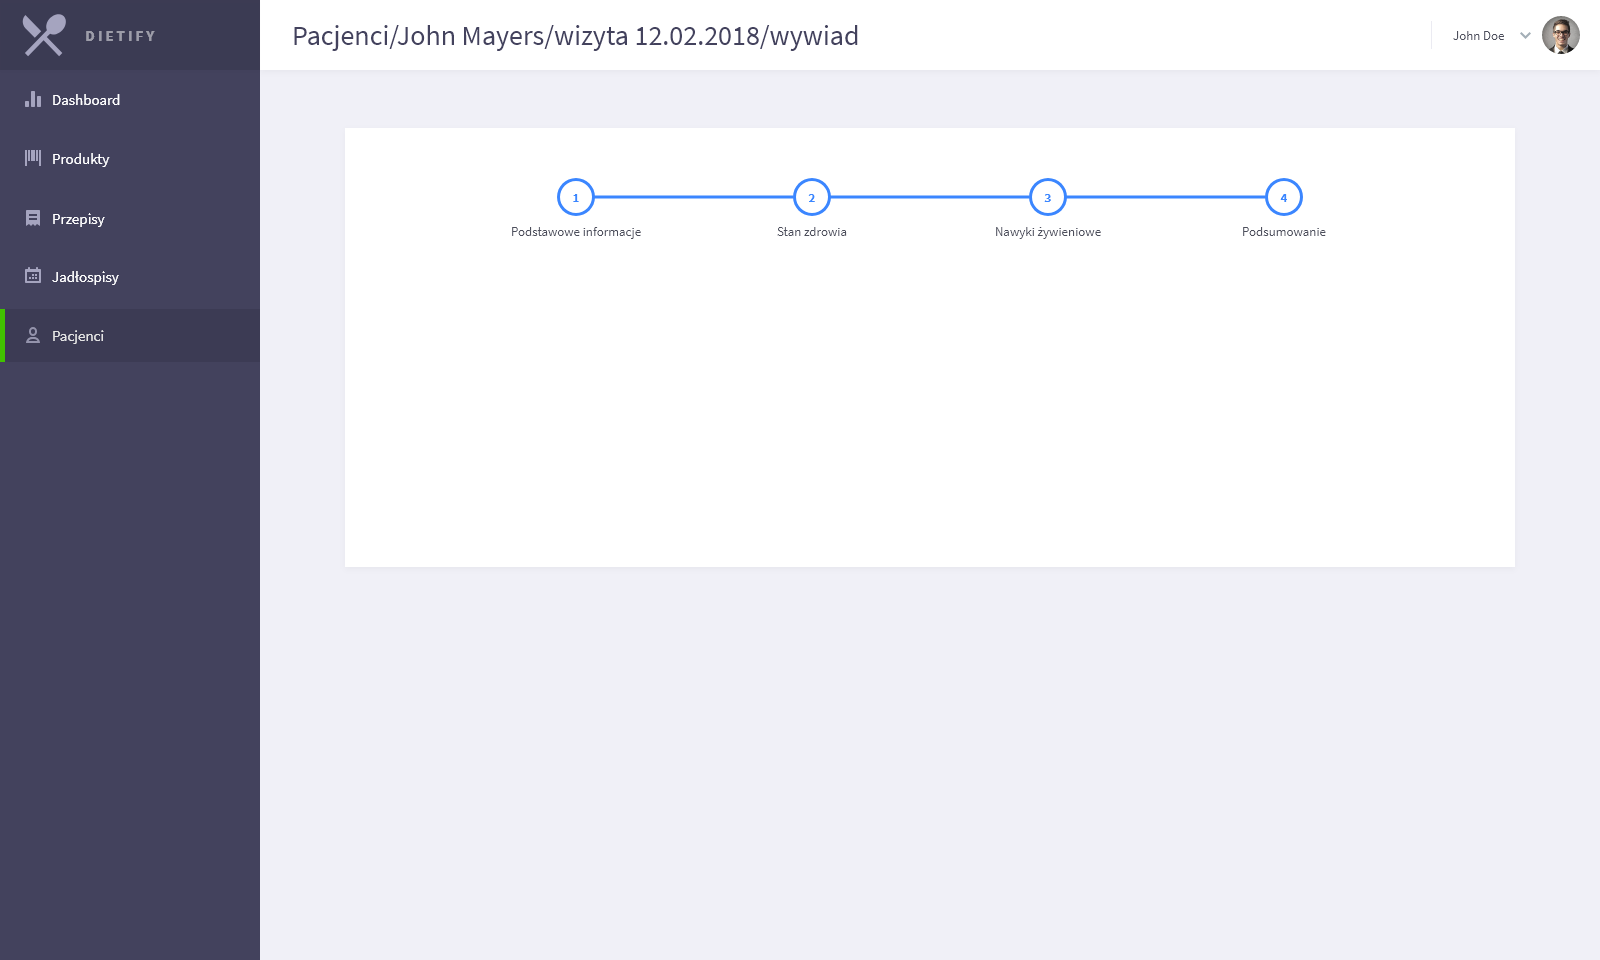
\includegraphics[width=0.9\textwidth]{img/mockups/mockup16.png}
        \caption{Mockup16 (opr.wł).}\label{rysunek:mockup16}
    \end{figure}
\end{minipage}

\section{Baza danych}
\todo{diagram erd}
\todo{jdl}
\todo{mikroserwisy}

\thispagestyle{normal}
